\documentclass {CSEThesis}

% \usepackage[showframe , margin=1in , top = 0.5in]{geometry}
 
\usepackage[hidelinks]{hyperref}
\usepackage{amsmath}        % Extra math definitions
\usepackage{graphics}       % PostScript figures
\usepackage{setspace}       % 1.5 spacing
%\usepackage{psfig,epsfig}
\usepackage{multicol}
\usepackage{subfigure}
\usepackage{hyperref}
\usepackage{epsfig,color}
\usepackage{titlesec}
\usepackage{float}
\usepackage[T1]{fontenc}
\usepackage[utf8]{inputenc}
\usepackage{amsmath}
\usepackage{amsfonts}
\usepackage{algpseudocode}
\usepackage{algorithm}
%% use this in your preamble
\usepackage{newunicodechar}
% \usepackage{caption}
% \usepackage{subcaption}
\newunicodechar{ff}{ff}
\newunicodechar{fi}{fi} 
\newunicodechar{fl}{fl}
\newunicodechar{ffi}{ffi}
\newunicodechar{ffl}{ffl}
%% end of common ligatures
% Custom packages
%\usepackage[first]{datestamp}   % Datestamp on first page of each chapter
\titleformat{\chapter}[display]   
{\normalfont\huge\bfseries}{\chaptertitlename\ \thechapter}{20pt}{\Huge}   
\titlespacing*{\chapter}{0pt}{-50pt}{40pt}

\usepackage{color}

\btptitle = {Railway Scheduling Using Reinforcement Learning} % { and } are needed around your name
\name = {Arpit Singh}          % and other feilds. don't remove.
\rollno = {111601031}
\email = {111601031@smail.iitpkd.ac.in}
\guide = {Dr. Chandra Shekar Lakshminarayanan}


\begin{document}
\let\cleardoublepage\clearpage
\begin{titlepage}
    \begin{center}
    \textheight 15.5in \textwidth 12.5in {\large\sf  \textbf{\the\btptitle}}\\[12ex]
    {\small{\textsl{ \textbf{A Project Report Submitted \\
    in Partial Fulfillment of the Requirements \\
    for the Degree of \\
    [3ex]\small \bf Bachelor of Technology}}}}\\
    [16ex] \emph{by}
    \\[2ex]
    {\sf \sf \textbf{\the\name}\\
                 (\the\rollno)}\\[1ex]
    \emph{under the guidance of}\\[2ex]
    {\sf \bf \the\guide} \\[7ex]
    
    \vspace{1.2in}
    
     \begin{figure}[!h]
    \centering
     
\includegraphics[width=0.15\textwidth]{IITPkdFullLogoColor}
     \end{figure}
    
    
    
    {\small\bf DEPARTMENT OF COMPUTER SCIENCE AND ENGINEERING}  \\[1ex]
    %{\small \bf{INDIAN INSTITUTE OF TECHNOLOGY PALAKKAD}}
    %\\[2ex]
    %
    %  {\color{red} \hrule height 0.5ex}
    % \vskip 1ex
    % May \the\year 
    \end{center}
    \end{titlepage}
    
\tableofcontents 
% \voffset=-0.8in
\addcontentsline{toc}{chapter}{List of Figures}
\listoffigures 

\pagenumbering{arabic}
\def\headrulehook{\color{black}}      % Color the header rule

%========== Chapters
% \voffset = -0.2in;
% \typeout{}
% \chapter*{\centering Acknowledgements}
\quad Write acknowledgements, if your want to.


% \cleardoublepage
\typeout{}
\titleformat{\chapter}[display]{\normalfont\Large\bfseries}{}{11pt}{\Huge}
\chapter{Introduction}
\pagenumbering{arabic}\hspace{3mm}


The aim is to work on an algorithm for scheduling
bidirectional railway lines (both single- and multi-track) using a
framework of Reinforcement Learning. Given deterministic arrival/departure times for
 all the trains on the lines, their initial positions, 
 priority and halt times, traversal times, deciding on track allocations is a 
 job shop scheduling problem (NP Complete ). However, 
 due to the stochastic nature of the delays, 
 the track allocation decisions have to be made in a dynamic manner, 
 while minimising the total priority-weighted delay. 
 This makes the underlying problem one of decision making in of 
 stochastic event driven systems. 
The primary advantage of the proposed algorithm compared to
exact approaches is its scalability, and compared to heuristic
approaches is its solution quality.Improved solution quality is obtained because
of the inherent adaptability of reinforcement learning to specific
problem instances.

\vspace{\baselineskip}
This report is organised in 4 main chapters.Chapter 2 discusses the problem statement in length, 
Chapter 3 discusses the implementation of the simulator, Chapter 4 discusses the algorithm details and 
Chapter 5 discusses the experiments and results. Last chapter discusses about the future course of the project.

\cleardoublepage 
\typeout{}
% \newgeometry{margin = 1in , top = 0in}
% \voffset=-0.in
\chapter{Problem Statement}
% \titleformat{\section}{\large\bfseries}{\thesection}{1em}{\ }
\section{Indian Railways}
\pagenumbering{arabic}\hspace{3mm}

Let us first describe the nature of the railway system in this country. 
The Indian railway network is designed to consist of long ‘lines’ (a string of stations),
which connect with each other at ‘junction’ stations. Each station is composed 
of one or more parallel \textbf{tracks}, which may be associated with a fixed direction of 
traffic, or they could be bidirectional. Similarly, there are one or more tracks 
between each neighbouring pair of stations. These tracks are typically referred 
to as \textbf{sections}, in order to differentiate them from tracks actually at a station. 
The section tracks can also be unidirectional (fixed direction of train movement)
 or bidirectional. The Indian network typically consists of sections with one or two tracks. 
\\
\\
 \begin{figure}[H]
    \centering
    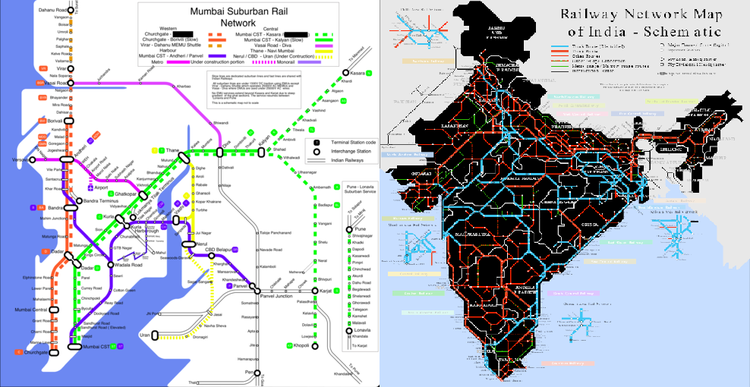
\includegraphics[width=0.8\textwidth]{Railways_pic}
    \caption{The line and junction topology of railway networks in India \cite{WEBSITE:1}. }
    \label{image-myimage}
\end{figure}

The approach we are focussing on now deals with linear railway 
networks with multiple parallel tracks, of the type shown in figure 2.2. This
restriction on topology is reasonable because rail networks are
designed in the form of multi-station linear arcs connected
at junction stations.

\begin{figure}[H]
    \centering
    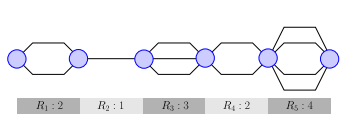
\includegraphics[width=0.4\textwidth]{report1}
    \caption{Linear Railway Lines \cite{ARTICLE:1}. }
    \label{image-myimage}
\end{figure}

\section{Railway Scheduling Problem}
\subsection{Scheduling}
A specific problem instance begins by defining the resources
on the railway line, as given by the number of stations, their
order, and the number of parallel tracks (both at each station
and between two neighbouring stations). Besides resource level information, 
train movements over the scheduling horizon must be described in one of two ways.
\begin{itemize}
    \item To define a reference timetable which gives the desired arrival
    and departure time of each train at each station.
    \item To provide the earliest movement times from their
    current locations (or origin stations), followed by the minimum
    running times (on track sections between stations) and halt
    times (at stations) up to the destinations.
\end{itemize}

\vspace{0.2cm}

Note that the running
and halt times can be completely heterogeneous: each train
may have a different running/halt time in each resource,
depending on the length of track, the type of halt, and the
type of locomotive.

\vspace{0.2cm}
Timetabling refers to an offline planning problem for a railway network.
\textbf{Given a set of trains and their origins and destinations (with or without a fixed route),
 the goal is to assign track resources for each train for a fixed time period, 
 such that they all complete their journeys without conflicts.}

 \vspace{0.2cm}
 Such a timetable may be infeasible if the desired arrival and
departure times violate the track usage rules defined earlier.
The task of the scheduling algorithm is to adjust the arrival
and departure times such that all rules are satisfied, while
minimizing an objective called priority-weighted delay. This schedule
is to be computed for all trains up to their destinations.

\vspace{0.2cm}
The railway problem has been shown in literature to be a \textbf{‘blocking’ version of the 
Job Shop Scheduling Problem (JSSP)}, where the job (train) must wait in the current resource 
(track) until the next resource is freed (there is no buffer for storing jobs between 
two resources). This version of the JSSP is also \textbf{NP complete}, with the result that 
exact solutions require an exponential amount of time for computation.
\vspace{1in}
\subsection{Rescheduling}

Another problem is that of rescheduling.
Rescheduling is the online counterpart of the timetabling problem , 
where the goal is to recover from a disruption to the timetable, 
caused by delays or faults. The mathematical differences are found in two aspects. 
\begin{itemize}
\item The goal is to return to the original timetable using built-in slack times, 
instead of defining the timetable itself. 
This implies that the objective function would focus on minimizing delays to 
trains with respect to the timetable, or the time required for deviations to the smoothed out. 
\item The online nature of the problem implies that there is very limited time 
available to compute solutions, and that sub-optimal but reasonably efficient 
solutions are acceptable. 
\end{itemize}

% \section{Time Table Scheduling problem}


\cleardoublepage 
\typeout{}

\typeout{}
\chapter{Simulator Implementation}
The integrated reinforcement learning algorithm to derive the whole schedule is driven
by a discrete event simulator. There are already some railway simulators like \textbf{OpenTrack} \cite{WEBSITE:2} and \textbf{RailML}\cite{WEBSITE:3} but they
would be useful for the final analysis of the results. Once we have the desired timetable then we can use these 
simulator softwares to determine the quality of solution. But for the implementation of the 
algorithm we have to implement the simulator on own.

\section {Railway simulator}
\subsection{Requirement}
The simulator is supposed to be robust enough that it can run both toy and real life 
examples. 
The simulator is suppose to run through several episodes during training and hence need 
to be efficient. At the
beginning of every episode, the initial locations of all the trains
are reset to their original values. It is assumed that trains that have not yet started, 
or have finished their journeys, do not
occupy any of the tracks. Following the train-to-resource mapping, 
the simulator creates a list of events for processing, one
corresponding to each train (whether already running or yet to
start its journey). Each event in the list contains the following
information: the time at which to process the event, the train to
which it corresponds, the resource where the train is currently
located, the last observed state-action pair for the train (empty
if the train is yet to start), and the direction of the train journey. 

\vspace{\baselineskip}
At each step, the algorithm moves the simulation clock to
the earliest time stamp in the event list. If multiple events are to
be processed at the same time stamp, they are handled sequentially. We are for now 
not focussing on how to avoid deadlock, but instead if we get into deadlock, we will detect and give huge
negative reward and the RL algorithm is suppose to avoid deadlock on it's own.


\subsection{Implementation}
There are two components to railway simulator :
\begin{enumerate}
    \item Underlying Railway Network. 
    \item Trains and the simulation of there movements.
\end{enumerate}

For the implementation of the railway network we can use \textbf{NetworkX}\cite{WEBSITE:4} package of python.
\textbf{NetworkX is a Python package for the creation, manipulation,
and study of the structure, dynamics, and functions of complex networks.}
\vspace{1.5cm}

Once the network is ready we have to simulate movement of each train over the network. For 
that we can use \textbf{SimPy}\cite{WEBSITE:5} package of python. \textbf{SimPy is a process-based discrete-event simulation framework based on standard Python}.
In this we can model each train as the separate process and network as the resource. We can 
model the movement of trains using this package. We yield events when the train starts from some station and once 
the train reaches the next station, event is yielded and then we can process accordingly. So whole simulation is done 
by generating events at points where the algorithm is supposed to take action.

\vspace{\baselineskip}
Once the railway network is created, train class is used to create different instances
of the trains running over the network.

% =============================================================================================================
\section{Implementation Details}

This section focuses on the implementation details of the railway simulator. Whole
implementation of railway simulator is captured by the flow diagram below. It consists of 
different modules, which in turn are made of different components. First we will have a overview of
each of the modules and its components and then move on to study them in detail. Whole code base is in 
repository \cite{WEBSITE:6}

\begin{figure}[h]
    \centering
    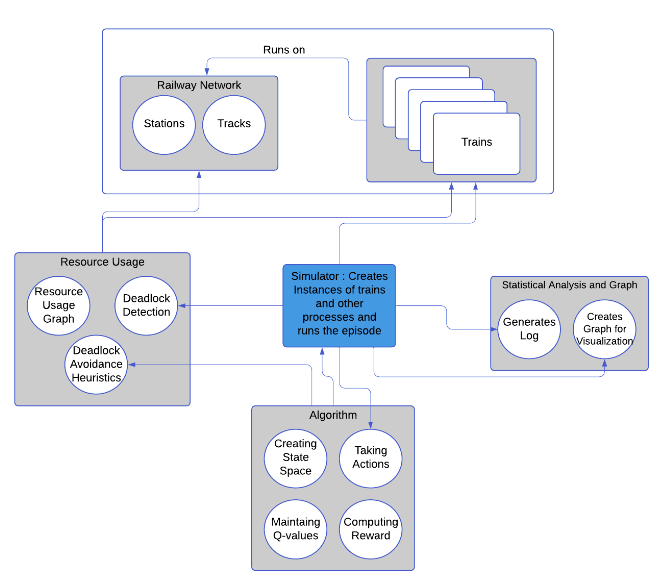
\includegraphics[width=1.0\textwidth]{Implementation}
    \caption{ Flow chart summarizing the implementation of railway simulator.  }
    \label{image-myimage1}
\end{figure}


\subsection{Modules and its components}
\begin{enumerate}
\item \textbf{Railway network and trains}

This is the main module that contains the basic architecture of railway network and the 
trains. Railway network consists of two basic components :-
\begin{itemize}
\item \textbf{Stations} : Stations in the railway network (synonymous to nodes in the network).
\item \textbf{Tracks} : Tracks connecting the stations (synonymous to edges in the network).
\end{itemize}
Once the railway network is created, train class (implemented as component) is used to create different instances
of the trains running over the network.

\item \textbf{Statistical Analysis and Graphs}

This module is responsible for creating the logs and generating necessary graphs for visualization 
and analysis.

\item \textbf{Resource Usage}

Whole railway network (station and tracks connecting the stations) is treated as pool of resource.
 Trains are ones that use this resource as they reside either on the station or the track. 
There are only fixed number of trains that can reside on the station and the track at a time.
It is also possible for the train to wait for a resource to free up, as it is occupied by other
trains. \textbf{Resource Usage Graph} component is responsible for generating the graph which show
what all resources are occupied by the trains and for what all resources train is waiting. This can be useful in detecting
deadlock.


There is another problem of deadlock which the simulator can run in. We are going to discuss this problem 
in full length in the later sections.\textbf{ Deadlock detection} and \textbf{deadlock avoidance} components
are used for detecting and avoiding the deadlock in the systems.

\item \textbf{Algorithm}

This module implements the algorithm (Q-Learning or Deep Q-learning) that helps in learning
the schedule. Currently only two components are implemented, creating state space and 
choosing action based on heuristic in \cite{ARTICLE:2}. More algorithms will be added in the future.
\vspace{2cm}
\item \textbf{Simulator}

This is one of the most important module that is responsible for creating all the processes 
that runs the simulator. It creates the environment and then invokes all the processes, then it handles 
further processing. Because of this module, we can add more modules in the future to the existing system.

\end{enumerate}

% =================================================================================================
\section{Rail Network and Train}

This module is responsible for creating the underlying railway network and the trains that run on 
these networks. Railway network module is implemented in \textbf{network.py} and train component is implemented in 
\textbf{train.py}.
\vspace{0.5cm}
\subsection {Mathematical model}
This mathematical model is from \cite{ARTICLE:2}. The railway network is modelled as a graph
$ \mathcal{G}( \mathcal{N} ,\mathcal{E})$ where $\mathcal{N}$ denotes the set of all nodes, and 
$\mathcal{E}$ denotes
the set of all edges. A set of vehicles $\mathcal{V}$ is to be scheduled
through this network, which implies that vehicles $v_i \in \mathcal{V}$
must be allotted time slots at successive nodes and edges,
such that they can move from their respective origins to
destinations via predefined routes (sequence of nodes). Each
pair of nodes is connected by at most one edge, and thus
routes also define the sequence of edges to be traversed.
Each node $n_j \in \mathcal{N}$ and edge $e_k \in \mathcal{E}$ is assumed to be
composed of one or more parallel (equivalent) resources,
denoted by $r_{m}^{nj}$ and $r_{p}^{ek}$ respectively, where $m \in \{1, \ldots R^{n}_{j}\}$
and $p \in \{1, \ldots R^{e}_{k}\}$.

\vspace{0.25cm}
Let us define the arrival time of a vehicle $v_i$ at node $n_j$ by
$t_{i}^{a} (n_j)$, and its departure time to be $t^{d}_{i} (n_j )$. Complementarily,
the arrival time to and departure time from an edge $e_k$ is
denoted by $t^{a}_{i} (e_k )$ and $t^{d}_{i} (e_k )$ respectively. If $e_k$ is traversed
upon leaving $n_j$ , then $t^{a}_{i}(e_k) = t^{d}_{i} (n_j )$. If the next node
after $e_k$ is $n_{j}^{'}$ , then $t^{d}_{i} (e_k ) = t^{a}_{i} (n_{j}^{'} )$. For simplicity, it is
assumed that all parallel resources at a node are accessible
from all resources at adjoining edges. Finally, we define the
binary variables $b^{nj}_{m}(i)$ and $b_{p}^{ek}(i)$ to be equal to 1 if $v_i$ is
allocated to resources $r_{m}^{nj}$ and $r_{p}^{ek}$ at respective nodes or
edges, and 0 otherwise. Each vehicle $v_i$ has an earliest start
time on its journey (arrival time at first node) given
by $T_i$ , and its computed finishing time (departure from last
node) is denoted by $f_i$ . Its minimum halt time at node $n_j$
is given by $H_i (n_j )$, and minimum travel time on edge $e_k$ is
given by $W_i (e_k )$.

\vspace{0.25cm}
Time constraints, $$t^{d}_{i} (n_{j} ) - t^{a}_{i} (n_{j} ) \geq H_{i} (n_{j} )$$
$$t^{d}_{i} (e_{k} ) - t^{a}_{i} (e_{k} ) \geq W_{i} (e_{k} )$$

Resource Contraints,
$$\sum_{m} b_{m}^{nj}(i) = 1$$
$$\sum_{m} b_{m}^{ek}(i) = 1$$

\subsection{Railway Network}


Railway network consists of two building blocks \textbf{Stations} and \textbf{Tracks} that connect
stations. All the fields of tracks and stations are given in the diagram below. Railway network is a weighted 
networkx graph where nodes are stations (Station class is added as attribute to the node) and edges are 
tracks running between stations (Track class is added as attribute to the edge). Input is given using two
separate text files, one corresponding to tracks and other corresponding to stations. More detailed info is 
in repository.


\begin{figure}[h]
    \centering
    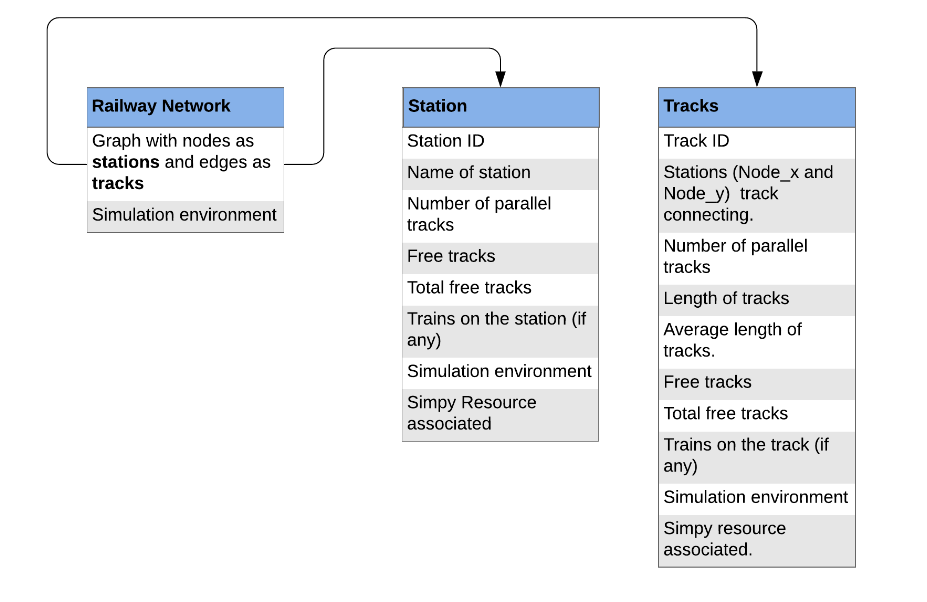
\includegraphics[width=1.0\textwidth]{Rail_train}
    \caption{ Railway Network framework }
    \label{image-myimage2}
\end{figure}

\subsection{Trains}
There are multiple trains running in the network at a time. Train class defines all the variables and methods
of this class and simulator uses this class to create process corresponding to each train (more details in simulator 
section).

\vspace{0.25cm}
Train movements over the scheduling horizon must be described in one of two ways. The first option is
to define a reference timetable which gives the desired arrival
and departure time of each train at each station. The second
option is to provide the earliest movement times from their
current locations (or origin stations), followed by the minimum
running times (on track sections between stations) and halt
times (at stations) up to the destinations. Note that the running
and halt times can be completely heterogeneous: each train
may have a different running/halt time in each resource,
depending on the length of track, the type of halt, and the
type of locomotive. The timetable can be derived by adding
the running and halt times of each train to the current time.

\begin{figure}[h]
    \centering
    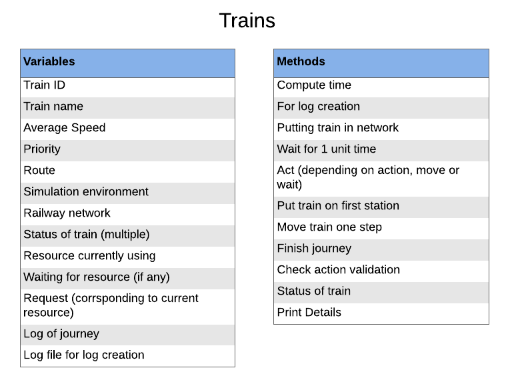
\includegraphics[width=0.8\textwidth]{train}
    \caption{ Train Variables and methods }
    \label{image-myimage3}
\end{figure}

Variables in the train class are self understood. Following are the explanation and implementation details of 
the method. For more details look into the repository where explicit documentation is given.
\begin{enumerate}
\item \textbf{Compute Time} : To calculate the travel time of the train between two stations.
\item \textbf{Log Creation} : To create log corresponding to important events for each train.
\item \textbf{Put train in network} : This method puts the train in the network and generates an event 
                                    corresponding to start time of the train. After start time, train movement is 
                                    controlled using \textbf{Act} method.
\item \textbf{Wait} : To make train wait for predefined unit of time.
\item \textbf{Act} : This method takes one argument, either to move the train or wait. Depending on the 
                    argument, specified action is taken.
\item \textbf{Put train on first station} : This method tries to put the train onto first station and thus 
                            initiating the journey of the train. It may be possible, that the station is not 
                            free, in which case the move is invalid or it waits till the resource is freed.
\item \textbf{Move train one step} : Move the train one step. If the train is on the station, then it will try to 
                                depart to the next track or if the train is on track, then it will try to arrive at the 
                                next station.
\item \textbf{Finish journey} : This method is used when the train is at the last station and it has to 
                                free the last resource.
\item \textbf{Check action validation} : Check wether the given action (move or wait) is valid for the current status of the train.
\item \textbf{Status of train} : To give the current status of the train.
\item \textbf{Print details} : To print the details of the train.
\end{enumerate}

Trains need action only for the following events :
\begin{enumerate}
\item If a train is standing at a station, the event processing time 
    corresponds to the earliest time at which the train can depart,   
    as defined by its minimum halt time at the station and by any     
    departure time constraints enforced for passenger convenience.
\item If it is running between two stations, the event processing time        
    corresponds to the earliest time at which it can arrive at the         
    next station, as defined by the length of the track and the train      
    running speed.

\item  If the train is yet to start, the event processing                      
    time is the time at which it is expected at the starting station. This event is created 
    by \textit{put train in network} method. Once this event is generated, then \textit{put train on 
    first station} is used to put the train on the first station.

\end{enumerate}


Once the train process is running, it is in one of the following states :
\begin {enumerate}
\item Train is not yet started.
\item Train is running in the network.
\item Train has reached the destination( final station in journey) but the resource is not yet freed.
\item Train has completed journey and released all the resources.
\end {enumerate}

This status is used by create statistics process, that terminates the simulation if all the trains have completed it's 
journey.




%===========================================================================================
\section{Statistical Analysis and Graph}

This module is responsible for creating the statistics and Graphs for visulalization and analysis. This 
module proves to be very important for debugging. Currently only two components are implemented but more
can be implemented in future as per the need.

\subsection{Log generatotion}
This component generates all the log in the system. There are two sets of log. One corresponding to each train that gives 
info about the status of the train at different times during the simulation. Another generates log corresponding 
to the status of the network, how many trains are there in the network and wether the network is in deadlock or not. All 
logs are generated and put in the folder \textbf{Log}.

\subsection{Graphs for visulalization}
This component creates graph for visualization, while the simulation is running. Amount of detail 
we want in the graph can be controlled using different arguments. Note that this component slows down the simulation,
so when the learning algorithm is running we can turn off this component.

\subsection{Details of the image} 
Each station is represented by node and each track is represented by edge
connecting these nodes. There can be more than one railway line on station or track, so the width of the 
nodes or the edges is directly propotional to the number of railway lines on that resource. How many lines 
are free on a given resource, that is encoded using the labels (on nodes and edges) and light green color. 
Each train running in the network is color coded. If more than 8 trains are running in the network, then all the trains
will have the same color (then image just shows the resource level information about each resource in the network).
We can control the amount of detail in the network by passing different arguments. For more details, look into the 
code repository. 


\begin{figure}[h]
    \centering
    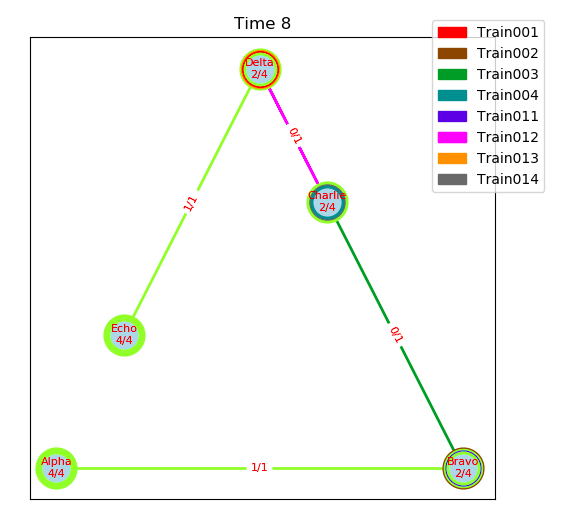
\includegraphics[width=0.5\textwidth]{graph}
    \caption{ Network with trains color coded.  }
    \label{image-myimage5}
\end{figure}

\begin{figure}[H]
    \centering
    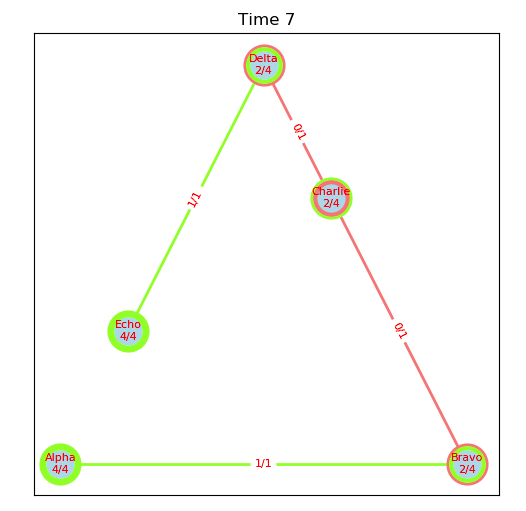
\includegraphics[width=0.5\textwidth]{graph2}
    \caption{ Network showing just what all resources are free.  }
    \label{image-myimage6}
\end{figure}

%========================================================================================
\section{Resource Usage}

This module monitors the resource usage in the network. This module is also responsible for detecting deadlock and 
implementing heuristic that avoids deadlock upto certain extent (more details in the following sections). 
  
\subsection{Resource usage graph}
This component is responsible 
for creating graph, that shows which train is using which resource(track or station) and waiting for 
which resource(if any). Pink node corresponds to train, blue corresponds to stations and green corresponds 
to track. If a train is occupying a resource (station or track), then we have an arrow from resource to train.
If a train is waiting for a resource to be freed, then we have the arrow from train to resource.

\begin{figure}[h]
    \centering
    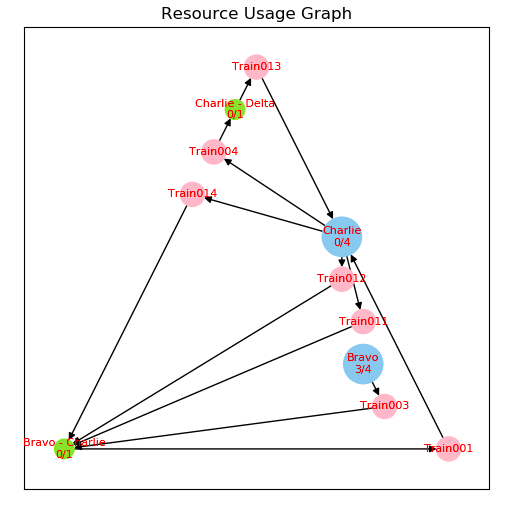
\includegraphics[width=0.65\textwidth]{resource}
    \caption{ Resource usage in the network.  }
    \label{image-myimage6}
\end{figure}

\subsection{Deadlock detection}
Simulator encounters deadlock if the next chosen move is
infeasible because $(i)$ vehicle $v$ finds all resources at the
next node occupied by other vehicles, and (ii) these other
vehicles can only release their current resources if they
move into the resource currently occupied by $v$. 
In the figure below, there are four trains at station Charlie, one train on track Delta-Charlie, trying to move to station Charlie 
and one train at track Charlie-Bravo, trying to move to station Charlie. Since no trains can move in this scenario, so it is in deadlock.

\begin{figure}[h]
    \centering
    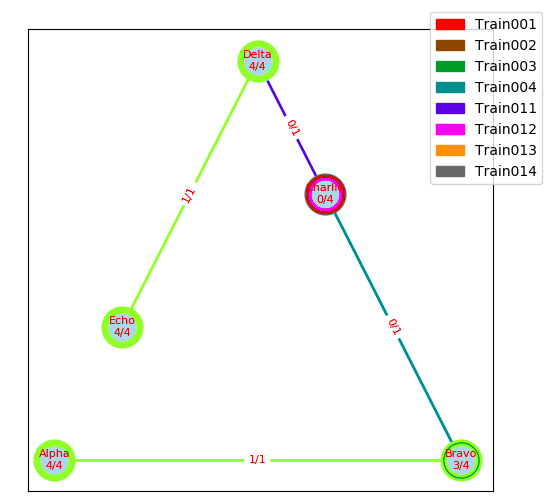
\includegraphics[width=0.65\textwidth]{deadlock}
    \caption{ Deadlock near station Charlie.  }
    \label{image-myimage6}
\end{figure}

In this simulator, each resource (station or track) is having multiple instances
(lines). If each resource have only one instance, then deadlock can be detected by cycle in resource 
usage graph. But since, each resource is having multiple instances, we have to use banker's algorithm to detect deadlock.
Once the deadlock is detected, simulation is terminated and huge negative reward is given.

\subsubsection{Banker's algorithm}

This algorithm is originally used to avoid deadlock. We are going to modify this to detect deadlock.
Here, trains are treated as processes and tracks or stations are treated as resources.
Let's $n$ be the number of processes (trains) and $m$ be the number of resource categories (number of stations and tracks in 
the network). The banker's algorithm relies on several key data structures:
\begin{enumerate}
\item $Available[m]$ indicates how many resources are currently available of each type.
\item $Max[n][m]$ indicates the maximum demand of each process of each resource.
\item $Allocation[n][m]$ indicates number of each resource category allocated to each process.
\item $Need[n][m]$ indicates the remaining resources needed of each type for each process. 
( Note that $Need[i][j] = Max[i][j] - Allocation[i][j]$   $\forall i, j$. )
\end{enumerate}

This algorithm determines if the current state of a system is safe, according to the following steps:
\begin{enumerate}
\item Let Work and Finish be vectors of length $m$ and $n$ respectively.
\begin{itemize}
\item Work is a working copy of the available resources, which will be modified during the analysis.
\item Finish is a vector of booleans indicating whether a particular process can finish (or has finished so far in the analysis).
\item Initialize Work to Available, and Finish to false for all elements.
\end{itemize}
\item Find an $i$ such that both $(A)$ $Finish[ i ] == false$, and $(B)$ $Need[i] < Work$. This process has not finished, but could with the given available working set. If no such i exists, go to step 4.
\item Set $Work = Work + Allocation[i]$, and set $Finish[i]$ to $true$. This corresponds to process $i$ finishing up and releasing its resources back 
        into the work pool. Then loop back to step 2.
\item If $finish[i] == true$  $ \forall i$, then the state is a safe state, because a safe sequence has been found.
\end{enumerate}

This algorithm is used to avoid deadlock. 
In our case $Available$ is the number of resource instances (lines 
on stations or tracks) free. $Allocated$ is the number of resource instance (lines on station or tracks) occupied 
by the train and $Requested$ is the resource instance requested by the train. 
If we use $Max = Allocated + Requested$, then above can be used to \textbf{detect deadlock} in the system.

\vspace{0.25cm}
Another important question is when to use deadlock detection algorithm. If use it very frequently 
then it's waste of computation as most the time system will not be in deadlock. If we use it very less
then system may be in deadlock for long time. So we have to find some middle ground. Here, we are currently checking deadlock
after every 20 units of time, it may be changed in the future. If the system is in deadlock, then 
simulation is terminated.

% \vspace{5cm}
\subsection{Deadlock avoidance heuristic}
Multiple trains are running in the network. It is possible that multiple trains need action at a particular simulation time.
So we have to pick one of these trains, and take action (move or wait) corresponding to 
train. This is done using deadlock avoidance heuristic based on \cite{ARTICLE:2}.
Intuitively, pick the train which is in the most
congested resource first. The lower the number of free tracks
in a resource, the higher the congestion, and the earlier the
processing of a train occupying that resource. This way we can avoid deadlock upto certain extent.

\vspace{0.25cm}
This algorithm takes TRAINS\_NEEDING\_ACTION, which is a global variable consisting of all the trains
that need action at a particular time, as input and gives the name of the train that is suitable to 
take action as output. 

\subsubsection{Algorithm}
\begin{enumerate}

\item Find status of all trains (not yet started , running , at last station or completed journey) in  
    TRAINS\_NEEDING\_ACTION.
\item Remove all trains that have completed there journey since they don't need action and generate a warning in log 
    as such train should not be in TRAINS\_NEEDING\_ACTION.
\item If there is such a train which is on last station but not freed the resource, then return that train 
     and terminate the algorithm.
\item If there is a train that has not yet started and waiting to be put on first station, then 
     return that train and terminate the algorithm.
\item Now all the trains are running. Construct an array where each element is a tuple of size 5 and corresponds to trains in 
    the TRAINS\_NEEDING\_ACTION. Items in the tuple are : 
\begin{itemize}
\item Name of the train
\item Resource (track or station) it is occupying.
\item Congestion on the resource, given by number of occupied lines on the resource.
\item Priority of the resource, given by minimum of the priority of all trains on the resource. 
\item Priority of the train
\end{itemize}

\item Pick train which is on most congested resource. If there is one such unique train then return it and 
     and terminate the algorithm. If not, go to next step.
\item Out of trains chosen from step 6, pick train on resource with highest priority. If there is one train needing action on that resource 
     then return it and terminate algorithm. If not, go to next step.
\item Out of trains chosen from step 7, pick train with highest priority. If there are multiple train then choose any one randomly and return it. 
\end{enumerate}

%============================================================================
\section{Simulator}

This module is responsible for carrying out the whole simulation and
 putting all the components in place. The way it does this is by creating
 processes that interact with each other and runs the simulation.
 This module is implemented with the help 
 of simpy that helps to create different processes. SimPy is a discrete-event simulation 
 library. The behavior of active components (like trains, deadlock detection or creating graphs) 
 is modeled with processes. All processes live in an environment. They interact with the environment 
 and with each other via events (which is created by this module). Note all the processes are 
 running \textbf{concurrently}. At last, Simpy is using priority queue to 
 order the events. There is a clock in the environment and it is the simulator that runs the clock, 
 esentially running the simulation. 

\vspace{0.25cm}

Simulator module first create the network (with the help of railway network component) and then
the \textbf{environment} under which the simulation is carried out. Then it creates 
various processes that runs in this environment. The processes are : 
\begin{enumerate}
\item \textbf{Trains}

There are multiple trains which are running in the network. Each train is an instance of 
train class implemented in the train component. Simulator creates each train as a process. These
trains are running over the same resource pool (railway network) and simulator helps in scheduling and 
running each train. Each train have two actions, either to move or to wait and these 
actions are implemented using \textbf{choose action} process.

\item \textbf{Choose action}

This process always runs and take actions for each train in the network.
Initially there are no trains in the network. Simulator puts them at the initial station at approriate time 
(depending on the schedule train is following). Once the train is put in the network, each train is either to move to the next resource
(station or track) or wait for some time at the current resource (predefined to 1 unit time, can be altered). These actions
help the train to complete it's journey from source to destination.
There can be multiple trains that need action at the same time.
TRAINS\_NEEDING\_ACTION is a global variable, that keeps track of the trains that need action at current simulation
time. So there are two tasks at hand :
\begin{itemize}
\item Choose a train from TRAINS\_NEEDING\_ACTION for taking an action. In this simulator, we are 
    using deadlock detection heuristic based on \cite{ARTICLE:2} for picking the train. Essentially this heuristic breaks
    the tie when multiple trains are waiting for taking the action.

    \item Next step is to take the action, either to move or to wait. Choice of action depends on the state
    space of the train (discussed in detail in Algorithm section). We can also randomize this process by 
    choosing the action randomly with fixed probabilities.
\end{itemize}
\item \textbf{Deadlock detection}


This process is invoked after every predefined time (20 units) and checks if the network is in deadlock 
or not.\textbf{ Banker's Algorithm} is used as the deadlock detection algorithm (discussed in detail in 
resource usage module). If the network is in deadlock, then 
simulation of the current episode terminates.

\item \textbf{Create Statistics}

This process is invoked after every predefined time (20 units) and generates statistics about the current 
state of the network in the main log file (look at log generation component). The statistics include :
\begin{itemize}
\item Number of trains not yet started. 
\item Number of trains currently running in the network.
\item Number of trains that have completed their journey but the resource is not freed.
\item Number of trains the have completed their journey and all the resources are freed.    
\end{itemize}
If all the trains have completed their journey and all resources are freed then the simulation is terminated.
More statistics about the state of the network can be added in future.  

\item \textbf{Update Graph}

This process is responsible for creating the running GIF of the railway network and the trains running on
the network. It's purpose is only visualization that further helps in debugging and analysis.
\end{enumerate}

All these processes are run by the simulator. In future, more processes can be added with different 
functionality. All one has to do is to create a component and then the simulator will create a process
that runs the component.



\cleardoublepage
\chapter{Algorithm Details}

The principal goal of the algorithm is to compute
schedules for railway lines (either from scratch or from a given
starting state) while having comparable online computation requirements. 
Three challenges need to be overcome
to in order to achieve this objective

\begin{enumerate}
\item The algorithm must be able to handle different infrastructure and train service instances. 
\item It must scale to large, realistic railway lines.
\item It must manage simultaneously moving trains.
\end{enumerate}
The first challenge is addressed by defining a map
from the specific state of the instance to a generalised state
space of fixed size. The second challenge is handled by
decentralising the decisions for individual trains, and limiting
the feature vector to a fixed local horizon around each
train. Finally, the ordering of train moves is handled by
a discrete event simulator which picks the order using a
previously defined deadlock-avoidance heuristic. Each
component is described below.

\vspace{\baselineskip}
Note that this algorithm focuses on computing schedules for \textbf{railway lines \cite{ARTICLE:1} , \cite{ARTICLE:4} instead of railway networks}.
First we will define the algorithm, test it and then have a look at why it can't work in 
railway network setting and then try to expand the learning to the railway network.

\section{Generalised State Representation}
We compute the state space as a function of \textbf{local neighborhood} of each
train.
A state vector is computed for each train every time a
decision about its next move is to be computed. Relative to
the direction of motion, we define resources as being behind
(in the direction opposite to the direction of motion) or in
front (in the direction of motion) of the train. A user-defined
finite number of resources $ l_b $ behind each train and $ l_f $ in
front of each train are used for defining the state vector. These
are referred to as local resources. Including a few resources
behind the train in the state definition ensures that overtaking
opportunities for fast-moving trains are not missed. The total
number of local resources is ($ l_b + 1 + l_f $). 

\vspace{\baselineskip}
The entry in the state vector corresponding to each local
resource takes one of R integer values $ \{0, 1, 2,..., R-1\} $,
referred to as the status $S_r$ of resource $r$. Higher values
indicate higher congestion within the resource, and are driven
by the number of occupied tracks.
Let us define the number
of tracks in resource r to be equal to $N_r$, out of which $T_{r,c}$
tracks contain trains converging with (heading towards) the
current train, while $T_{r,d}$ tracks contain trains diverging from
(heading away from) the current train. Since at most one train
can occupy a given track, we note that $T_{r,c} + T_{r,d} < N_r$. The
mapping from track occupancy to resource status is,

$$ S_r = R - 1 - min(R - 1, \left \lceil{N_r - w_c T_{r,c} - w_d T_{r,d} }\right \rceil ).$$

Here, $0 \leq w_c$, $w_d \leq 1$ are weights that can de-emphasise
the effect of converging and diverging trains on the perceived
status of a resource.
\begin{figure}[h]
  \centering
  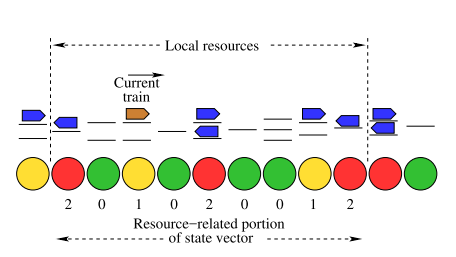
\includegraphics[width=0.6\textwidth]{report2}
  \caption{ Mapping train location and direction of movement to resource
  status, relative to the ‘current train’ \cite{ARTICLE:1}.  }
  \label{image-myimage}
\end{figure}

\vspace{\baselineskip}
In addition to the resource-related entries, the state includes
an entry for the priority of the current train.

\vspace{\baselineskip}
The complete state representation
used is a vector x of length ($l_b + l_f + 2$), including
the integer priority value and ($l_b + 1 + l_f$) entries for the status
of local resources. If we assume that the model accommodates
up to $P$ priority levels, the size of the state space is equal to
\textbf{($P * R^{l_b + 1 + l_f}$)}.\textbf{Note that this value does not depend on the
scale of the problem instance, in terms of the number of trains,
the lengths of their journeys, and the number of resources}.
One of the key advantage of using the local horizon as the state for the train is it's independence 
from the size of the problem instance. Another advantage is of \textbf{transfer learning} which we will see in later
sections.

\section{Action and Policy Definition}
The reinforcement learning procedure maps each state vector
 to a probability of choosing the action to be taken. In this
study, the choice of actions in any given state is binary, with
0 representing a decision to move the current train to the next
resource on its journey, and 1 representing a decision to halt
in the current resource for a predefined time period (1 minute
in this paper). If the train is halted, the decision-making
procedure is repeated after the time period elapses. The order
in which trains are selected for move/halt decision-making is given 
by deadlock avoidance heuristic in resource usage module. Let us assume that
a particular train occupying one track of some resource $r$ has
been selected, the state vector has been computed, and the
action (move or halt) is to be chosen. In addition to the state
vector, the choice of action is driven by the policy. Policy depends on the approach that we are going to use. 

\subsection{ $\epsilon$ - greedy policy}
Given a state, the two possible actions $a \in$  $\{$0 : move, 1 : halt$\}$ result in two unique
state-action pairs. Each state-action pair (x, a) is associated
with a Q-Value q(x, a) which quantifies its desirability. The higher the Q-Value, the higher the
desirability of the relevant pair. The $\epsilon$-greedy policy chooses
the greedy option (higher Q-Value) with probability ($1 - \epsilon$),
and a randomised action with probability $\epsilon$. The greedy choice
corresponds to \textbf{exploitation} of the learning so far, while the
randomised choice corresponds to \textbf{exploration} of the state-
action space. We are going to use this policy with standard Sarsa$(\lambda)$ the results of 
which are not good.

\subsection{Modified $\epsilon$ - greedy policy}

\begin{figure}[h]
    \centering
    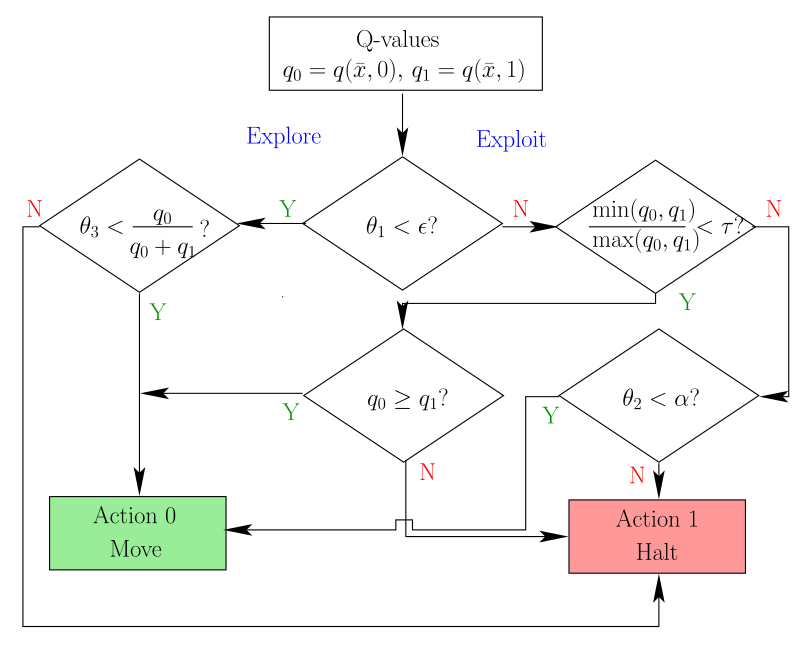
\includegraphics[width=0.7\textwidth]{policy}
    \caption{ Modified $ \epsilon$ - greedy policy \cite{ARTICLE:1}  }
    \label{image-myimage20}
\end{figure}

This is a modified version of the $\epsilon$ - greedy policy.
In exploration mode, the action is chosen with the
toss of a biased coin, based on the relative Q-Values $q_0$ and $q_1$
of the two actions. In the exploit mode, if $q_0 \approx q_1$
within a user-defined threshold $\tau$ , a further biased coin toss
is used to compute the action. The bias in this case is given
by a user-defined aggression parameter $\alpha$, which controls the
probability of choosing ‘move’ when $q_0 \approx q_1$ . If $q_0$ and $q_1$
are clearly separated, the action with the higher Q-Value is
chosen. The value of $\epsilon$ starts at 1 in the first training episode
and decreases as more episodes are completed. This moves
the policy gradually from exploration towards exploitation.

\vspace{\baselineskip}

The value of $\epsilon$ remains the same throughout the whole episode. In the first episode 
$\epsilon = 1$ and as the episode passes the value of epsilon decreases linearly upto min $\epsilon$,
after which it remains constant throughout the whole training.

\section{Objective Function}
A number of objective functions have been used in the
railway scheduling context, in order to achieve goals such
as delay reduction, passenger convenience, and timetable
robustness. One of the commonly used measures of
schedule quality is priority-weighted delay. A delay is
defined to be the non-negative difference between the time
of an event as computed by the algorithm, and the desired
time as specified by the timetable. The priority-weighted
average delay is the mean over all trains and all stations
of individual delays divided by train priorities. This quantity
is used as the objective function, but the algorithm can
accommodate other measures equally easily (for example,
a non-linear function of delays in order to increase fairness
of delay distribution).
$$ J = \frac{1}{N_{r,t}} \sum_{r,t} \frac{\delta_{r,t}}{P_t} $$
where $\delta_{r,t}$ is the delay for train t on departure from resource r,
$p_t$ is the priority of train t, and $N_{r,t}$ is the total number of
departures in the schedule. Note that this expression includes
all events for all trains, for their entire journey.

\section{Sarsa$(\lambda)$}
One of the typical algorithm is to use the objective function defined above as the negative of the reward. 
In that case, we will be having the reward at the end of each episode (terminal episode).
In each episode, each train is going through certain state-action pairs, forming a trajectory. And at the end
of each episode, we will get the reward. We can backpropogate the reward through this trajectory to learn
the Q-values. This learning is done using Sarsa($\lambda$).

\vspace{\baselineskip}
In Sarsa($\lambda$), we are using standard $\epsilon$ - greedy policy. This section discusses the forward view of 
Sarsa ($\lambda$) using eligibility traces. Q-values are updated using 
$$ Q_{t+1}(s,a) = Q_t(s,a) + \alpha\delta_te_t(s,a)  \;\; \forall(s,a)$$ 
where 
$$\delta_t = r_{t+1} + \gamma*Q_t(s_{t+1} , a_{t+1}) - Q_t(s_t ,a_t)$$
and 
\[
    e_t(s,a)=\left\{
                \begin{array}{ll}
                  \gamma\lambda e_{t-1}(s,a) + 1 \;\; if \; s=s_t \;\; and \; a=a_t\\
                  \gamma\lambda e_{t-1}(s,a) \;\;\;\;\;\;\;\; otherwise.\\
                \end{array}
              \right.
\]

Here, $\alpha$ is the learning rate, $\gamma$ is discount factor, $r_{t+1}$ is the reward (we have only 
one reward at the end of episode). Algorithm is given below.


\begin{figure}[!htb]
    \centering
    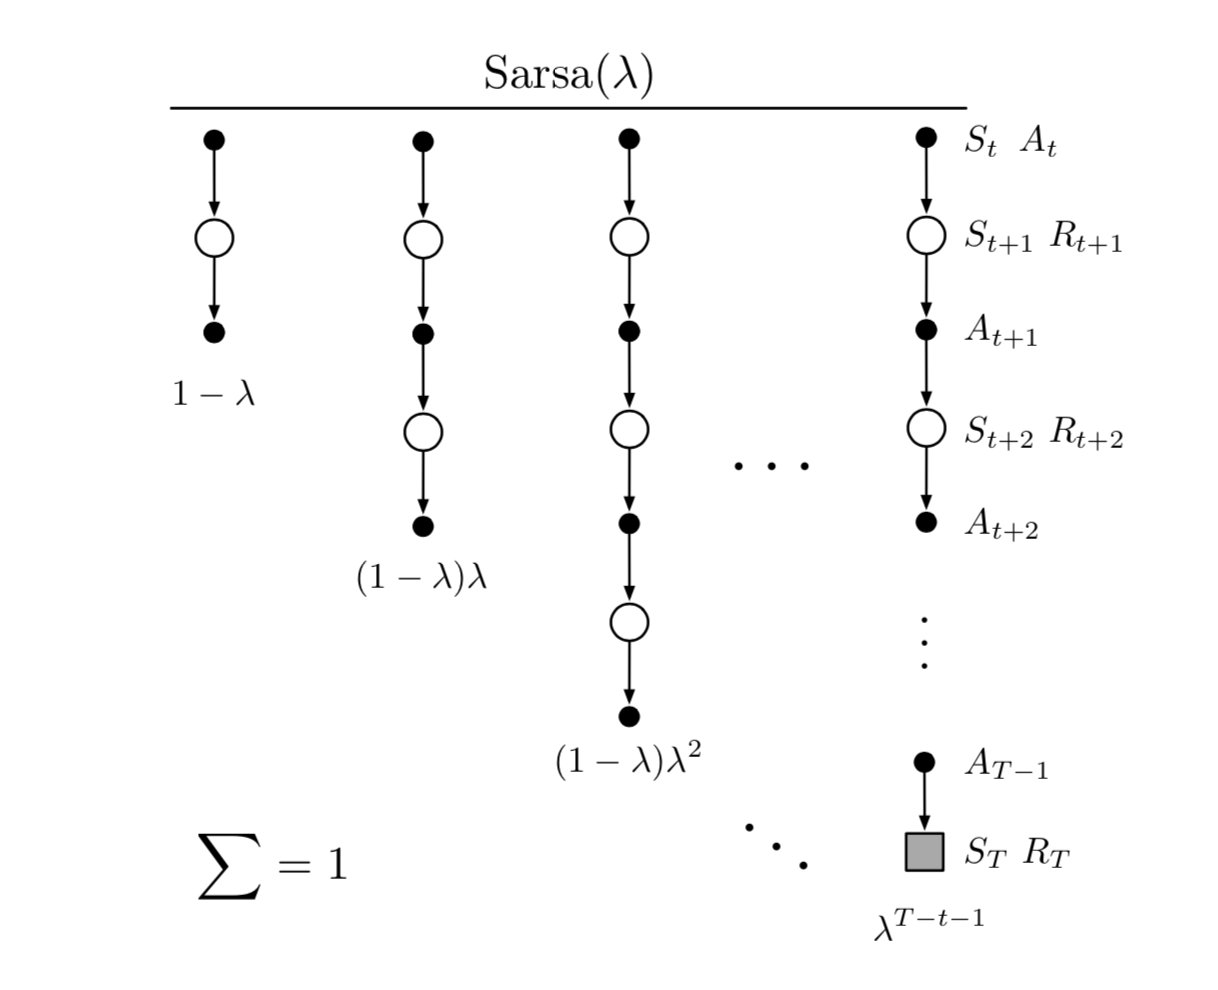
\includegraphics[width=0.7\textwidth]{backup_sarsa}
    \caption{ Sarsa($\lambda$)'s backup diagram \cite{BOOK:1} }
    \label{image-myimage20} 
\end{figure}

\begin{algorithm}[H]
\caption{ Sarsa Lambda \cite{BOOK:1} }
\begin{algorithmic}
\State Initialize $Q(s,a)$ arbitrarily and $e(s,a) = 0$ $\forall s,a$
\State Repeat (for each episode):
\State \;\;\;\;\;\;Initialize s,a    
\State \;\;\;\;\;\;Repeat (for each step of episode):
\State \;\;\;\;\;\;\;\;\;\;\;\; Take action $a$, observe $r$,$s'$
\State \;\;\;\;\;\;\;\;\;\;\;\; Choose $a'$ from $s'$ using $\epsilon$ - greedy policy
\State \;\;\;\;\;\;\;\;\;\;\;\; $\delta \gets r + \gamma Q(s',a') - Q(s,a)$
\State \;\;\;\;\;\;\;\;\;\;\;\; $e(s,a) \gets e(s,a) + 1$
\State \;\;\;\;\;\;\;\;\;\;\;\; For all $s$,$a$
\State \;\;\;\;\;\;\;\;\;\;\;\;\;\;\;\;\;\; $Q(s,a) \gets Q(s,a) + \alpha \delta e(s,a)$
\State \;\;\;\;\;\;\;\;\;\;\;\;\;\;\;\;\;\; $e(s,a) \gets \gamma \lambda e(s,a)$
\State \;\;\;\;\;\;\;\;\;\;\;\; $s \gets s'; a \gets a'$
\State \;\;\;\;\;\; until s is terminal
\end{algorithmic}
\end{algorithm}


\vspace{1.0in}
\section{Proxy reward}

The algorithm maintains a threshold of $J$ as the goal to be
achieved in each episode. This maximum acceptable level is
set to a proportion (1 + $\rho$) of the minimum $J$ observed thus
far, where $\rho > 0$ is a user-defined constant. The threshold
becomes tighter as the best known $J$ is improved upon during
learning. A reward of +1 (success) is given if the sum of the
priority-weighted delay is under the current threshold, and 0
(failure) either if it is over the threshold, or if the episode
enters deadlock and does not terminate.

\vspace{\baselineskip}
The Q-Values
are defined using the probability of success when an episode
passes through a given state-action pair. Instead of tracking
the entire sequence of state-action pairs in a given episode,
a binary indicator variable $b( x, a)$ corresponding to each pair
$( x, a)$ is set to TRUE whenever it is observed in a given
episode. Upon termination of the episode, the number of
successes (or failures) of all ( x, a) where $b( x, a) = TRUE$
are incremented by 1. The success probability $\sigma ( x, a)$ is
computed by dividing the number of +1 rewards associated
with the pair, by the total number of episodes that passed
through this pair. If $\epsilon_{x,a}$ is the number of all episodes that
passed through (x, a) at least once, and $\epsilon^{*}_{x,a}$ is the number of these 
that ended in success,
$$ 0 \leq \sigma(x,a) = \frac{\epsilon^{*}_{x,a}}{\epsilon_{x,a}} \leq 1$$

While $ \sigma ( x, a)$ provides a way to quantify the desirability
of a given state-action pair, it does not encapsulate the state
trajectory. On the other hand, a core tenet of reinforcement
learning is the back-propagation of rewards through the trajectory of state-action pairs (usually
upon episode termination).
However, in the current context, episodes can be very long,
reward is generated only upon episode termination, and state-
action pairs for multiple trains are generated simultaneously.
Therefore, $\sigma ( x, a)$ is used in as a \textbf{proxy reward}\cite{ARTICLE:1}.

We differ from the method mentioned in the paper by defining the Q-value differently.

\subsection{Prior}
In the paper, Q-value is defined as 
$$ q(x,a) = w\sigma(x,a) + (1-w)\sum_{m=1}^{M}\frac{\sigma(x'_m, a'_m)}{M }  $$
where w is a weighting factor between the success rate of a given pair, 
and the average success rate of its M neighbours. These M neighbours are not necessarily unique pairs, and thus 
neighbouring pairs that are more frequently observed have a greater contribution to the average value. 
 It is more like two step reward, in which Q-value is defined as the combination of success 
probability of current state-action pair and success probability of neighbors. Instead of looking at 
all the way down to trajectory, we are just looking at two steps of trajectory.

\subsection{Proposed}
We propose to have a Q-value that looks all the way down to the trajectory instead of 
two step reward functions. We propose Q-value as,
$$ q(x,a) = w\sigma(x,a) + (1-w)\sum_{m=1}^{M}\frac{q(x'_m, a'_m)}{M }  $$
where w is more like discount factor, that controls how far we are looking into the future. 
When $w = 1$, q-value just have immediate reward, when $w = 0$, Q-value is looking all the way into the future.
We will see later, that this small change changes the result significantly.
Again, these M neighbours are not necessarily unique pairs, and thus 
neighbouring pairs that are more frequently observed have a greater contribution to the average value.
We can also remove $w$ and put $\gamma$ as a discount factor, 
$$ q(x,a) = \sigma(x,a) + \gamma \sum_{m=1}^{M}\frac{q(x'_m, a'_m)}{M }  $$
One of the key advantage of defining Q-value like this,
is that we can use standard RL methods to learn the Q-values. Here, reward is the proxy reward that we 
have defined earlier and RL methods will try
to maximize this reward, getting tighter and tighter bounds on J and thus eventually decreasing 
the overall objective function. Although testing is done only for the first formula and second hypothesis 
still needs to be tested.

\section{Transfer Learning}
Transfer learning make use of the knowledge gained while solving one 
problem and applying it to a different but related problem. One of the key advantage of using 
proxy rewards is that we can transfer the knowledge gained while training one problem instance and then 
use it to test it on other problem instance. That means if we have a big problem instance, then once we train 
our algorithm on that problem instance, we can store its Q-value, and when training on other problem instance
we can use that Q-value as the starting point. Moreover, we can directly test using the stored Q-values.
The results of transfer learning is shown letter in the Experiment section.
\cleardoublepage
\typeout{}
\chapter {Experiments}

The algorithms as described above, is tested on three hypothetical problem instances. Description of all
the problem instances is defined in the next section. Two real life problem instances, Ajmer and Konkan 
railways still need to be tested but the hypothetical problem instances are comparable in size 
to the real life instances.

\section {Problem Instances}
\subsection{HYP-1}
The simple hypothetical instance HYP-1 consists of 8 trains
travelling 5 stations each. All trains are already
in the system at the start. Four trains heading left to right are
initially located in station Alpha, while the
others are in station Echo, heading right to left. Each station
contains 4 parallel tracks, and there is a single track between
stations. Only for HYP-1, the trains all have the same priority,
running times between stations, and halt times at stations.

\begin{figure}[h]
    \centering
    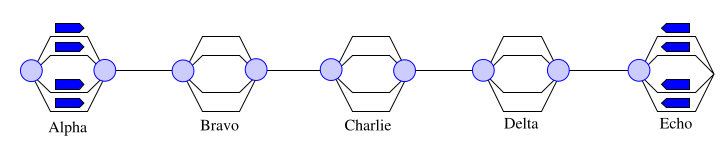
\includegraphics[width=0.7\textwidth]{Instance1}
    \caption{ HYP-1 }
    \label{image-myimage20}
\end{figure}

\subsection{HYP-2 \& HYP-3}
HYP-2 have 11 stations each having 3 tracks and each station is connected by a single bidirectional track.
The scheduling problem starts from the clean slate i.e. initially no train is in the network.
HYP-2 have 60 trains, 40 priority-1 train and 20 priority-2 train running. HYP-3 have double the number of trains 
i.e. 120 trains with 80 priority-1 train and 40 priority-2 train. Since the number of trains have 
doubled up, in HYP-3 each station have 4 tracks and single track is connecting these stations.

\begin{center}
    \begin{tabular}{ |c|c|c|c| } 
     \hline
     Name & Stns. & Trains (sorted by priority) & Events \\ 
     \hline
     HYP-1 & 5 & 8,0,0 & 40 \\
     \hline
     HYP-2 & 11 & 15,45,0 & 1320 \\
     \hline
     HYP-3 & 11 & 40,80,0 & 2640 \\ 
     \hline
    \end{tabular}
\end{center}

\section{Hyperparameters}
All results use a look-forward of $l_f = 6$ resources, and a
look-back of $l_b = 2$ resources. The status of each resource
takes one of three values: 0, 1, or 2 ($R = 3$). The weight on
converging trains is $w_c = 0.9$, while that on diverging trains
is $w_d = 1$. The maximum number of priority levels is $P = 3$.
In case of modified $\epsilon$ - greedy policy, the threshold for checking whether $q_0 \approx q_1$ 
is $\tau = 0.9$, and the aggression parameter is $\alpha = 0.9$. The
threshold for determining the maximum acceptable J is
$\rho = 0.25$. In case of Sarsa($\lambda$) , $\lambda = 0.9$ is choosen.

\vspace{\baselineskip}
Training is run for 500 episodes, where the $\epsilon$ is linearly reduced from 1 to 0.1 in 300 
episodes. Note, that the value of $\epsilon$ remains the same in each episode. Decrease in the value of 
$\epsilon$ is per episode basis.

\section {Results}
\subsection{Sarsa ($\lambda$) on HYP-1}

\begin{figure}[h]
    \centering
    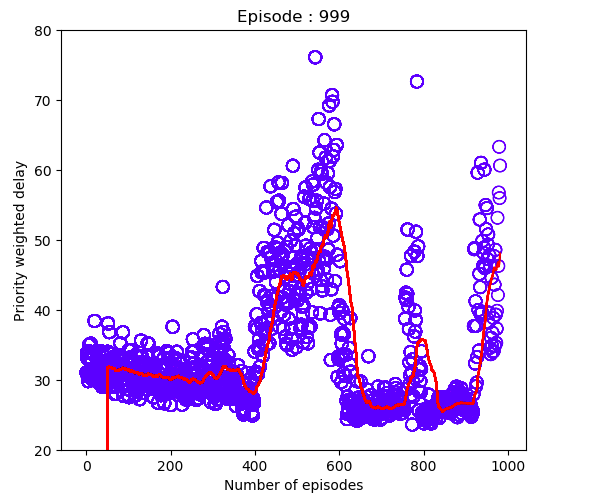
\includegraphics[width=0.7\textwidth]{Sarsa_HYP-1}
    \caption{ Priority weighted delay for Sarsa($\lambda$) on HYP-1 over 1000 episodes training}
    \label{image-myimage20}
\end{figure}

Sarsa($\lambda$) is not able to find an optimal schedule even for HYP-1. In the above plot, 
blue dots are the delay for one training episode, while red line is the running mean over the 
last 50 episodes.
The results of this algorithm is not good (in the next section) due to following reasons,
\begin{enumerate}
\item The back-propagation of rewards
      after the end of the episode is not possible, because the episode
can be very long.
\item In the trajecotry of a train, it is possible to visit the same state-action pair in loop leading to 
large accumulation of reward at that state-action pair, leading to extreme values.
\item Moreover, the magnitude of delays (and hence the theoretical
optimum value of $J$ ) is different from one problem instance
to another. Quantifying rewards directly in terms of delays
$\delta_{r,t}$ would create obstacles when transferring the learning from
one instance to another (\textbf{obstacle in transfer learning}).
\end{enumerate}

\subsection{Proposed work on HYP-1}
Q-values are initialised to 0.5 as they in some sense represent the probability of taking action either 
to move or to wait.
Training on the HYP-1 using the proposed approach, results in the convergence of Q-values. The Q-values 
decreased from around 35 to around 25. \textbf{Minimum is 23.58750}. Note the delay is only for those episodes that 
are successfully completed (not ending up in deadlock). Total number of episodes that ended up in deadlock 
are only 3 out of 500 episodes.

\begin{figure}[H]
    \centering
    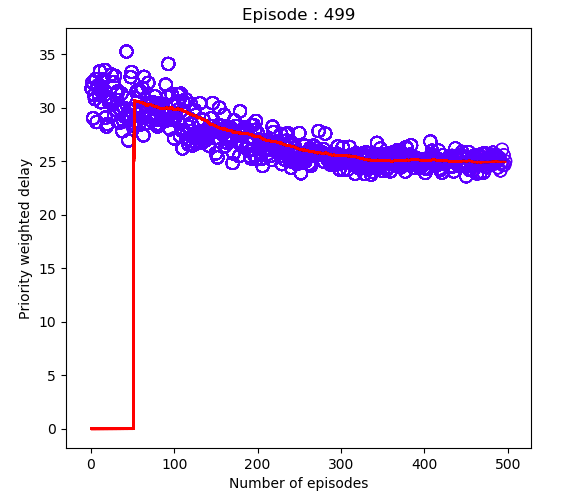
\includegraphics[width=0.7\textwidth]{/home/arpit/study/BTP/Results_image/HYP1/Approach2/1/delay}
    \caption{ Priority weighted delay for proposed approach on HYP-1 over 500 episodes training }
    \label{image-myimage20}
\end{figure}

The figure 11.4, shows time on the x-axis and
distance on the y-axis. Each solid line shows the trajectory of 
one train as it moves from one end of the line to the other. The
horizontal portions correspond to halts at stations, while the
inclined portions denote movement between stations. Since
there is a single track between successive stations and only
one train can occupy it at a time, inclined lines cannot cross
each other in a feasible schedule. The horizontal dotted lines
indicate specific tracks within station resources, and no two
solid lines are allowed to overlap within these tracks.

\begin{figure}[H]
    \centering
    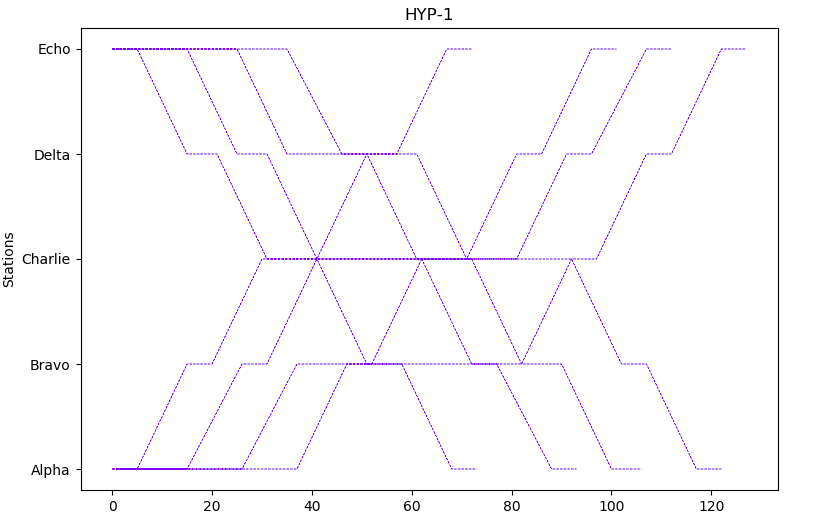
\includegraphics[width=0.7\textwidth]{/home/arpit/study/BTP/Results_image/HYP1/Approach2/1/train_running}
    \caption{ Schedule computed using proposed approach }
    \label{image-myimage20}
\end{figure}

\section{Training on HYP-2 \& HYP-3}
The toy instance like HYP-1 shows that the proposed
approach is able to learn Q-Values (and hence the policy for
choosing actions) at a small scale. However, when instances
of a realistic size and complexity are run with the same
initial Q-Values (0.5\%), they require a large number of training
instances to start producing feasible solutions. This happens
because the larger problem instances require several thousand
decisions to be made ‘correctly’ for successful completion.
When such decisions are made purely randomly, the instances
frequently end with trains in deadlock situations. 
So in order to speed up the training, the Q-values are initialized with the following 
heuristic.

\begin{center}
    \begin{tabular}{ |c|c|c|c| } 
     \hline
     \# & States Satisfying & Action & Init Q-values \\ 
     \hline
    1 & Next Resource is Full & Move & 0 \\
     & $ S_{r,next} = R-1 $ & Stop & 50\\
    
     2 & Atleast three consecutive resources are full & Move & 10 \\
     & $ S_r = S_{r+1} = S_{r+2} = R-1 $   & Stop & 15\\
    
     3 & Next Resource almost Full (R-2) & Move & 15 \\
     & Next but one is full (R-1) & Stop & 50 \\
    
     4 & Average status of upcoming resources & Move & 85 \\
     & is between 0.5 and 1.0 (moderately empty) & Stop & 90\\
     
     5 & Average status of upcoming resources & Move & 95 \\
      & is less than 0.25 (almost empty)  & Stop & 50\\
     \hline

    \end{tabular}
\end{center}

\section{Testing and transfer learning}

\begin{table}
\centering
\caption{Zero delay}    
    \begin{tabular}{ |c|c|c|c|c| } 
     \hline
     Train & Test & Minimum & Average & deadlock \\ 
     \hline
     HYP-2 & HYP-2 & 4.050 & 4.980 $\pm$ 0.590 & 0 \\
     & & 2.680 & 3.257 $\pm$ 0.501 & 0 \\
     \hline
     
     HYP-3 & HYP-2 & 3.089 & 4.080 $\pm$ 0.370 & 0 \\
     & & 2.709 & 4.184 $\pm$ 0.438 & 0 \\
     \hline

     HYP-2 & HYP-3 & 12.683 & 14.580 $\pm$ 1.058 & 16 \\
     & & 11.453 & 13.083 $\pm$ 1.164 & 6 \\
     \hline

     HYP-3 & HYP-3 & 11.855 & 12.954 $\pm$ 0.540 & 1 \\
     & & 11.438 & 12.734 $\pm$ 0.613 & 0 \\
     \hline
    \end{tabular}
\end{table}


\begin{table}
    \centering
    \caption{20\% delay}    
        \begin{tabular}{ |c|c|c|c|c| } 
         \hline
         Train & Test & Minimum & Average & deadlock \\ 
         \hline
         HYP-2 & HYP-2 & 9.591 & 11.388 $\pm$ 1.258 & 0 \\
         & & 8.386 & 10.261 $\pm$ 0.733 & 1 \\
         \hline
         
         HYP-3 & HYP-2 & 9.603 & 10.932 $\pm$ 0.881 & 3 \\
         & & 8.473 & 10.472 $\pm$ 0.792 & 1 \\
         \hline
    
         HYP-2 & HYP-3 & 26.882 & 31.955 $\pm$ 2.290 & 23 \\
         & & 27.734 & 30.141 $\pm$ 1.486 & 29 \\
         \hline
    
         HYP-3 & HYP-3 & 26.522 & 30.135 $\pm$ 1.649 & 3 \\
         & & 26.560 & 29.231 $\pm$ 1.723 & 1 \\
         \hline
        \end{tabular}
\end{table}
\cleardoublepage
\typeout{}
\chapter{Flatland Environment}

Since we have solved the problem of railway scheduling on a railway line,
we want to use the knowledge developed
so far and work on \textbf{railway scheduling on a railway network}.
Recently, AICrowd developed a flatland environment[11] to foster progress in multi-
agent reinforcement learning for any re-scheduling problem (RSP). They have
defined the railway network in a complete new setting using grid instead of graph. Future
course of the project is to work on more general problem of flatland (which can be used for
solve railway scheduling, transport management problems) and develop algorithms that can
solve scheduling problem over grid world having multiple agents.

\vspace{\baselineskip}
This chapter contains flatland environment specifications and discusses about the problem statement in 
detail. Flatland is usually a two-dimensional environment intended for multi-agent problems, 
in particular it should serve as a benchmark for many multi-agent reinforcement learning approaches.
The environment can host a broad array of diverse problems reaching from disease spreading to train traffic management.
The flatland environment is a two-dimensional grid in which many agents can be placed,
and each agent must solve one or more navigational tasks in the grid world.

\section{Environment}
Flatland is grid-like n-dimensional space of any size. 
A cell is the elementary element of the grid. 
The cell is defined as a location where any objects can be located at. 
The term agent is defined as an entity that can move within the grid and must solve tasks.
 An agent can move in any arbitrary direction on well-defined transitions from cells to cell.
 The cell where the agent is located at must have enough capacity to hold the agent on. 
 Every agent reserves exact one capacity or resource. 
 The capacity of a cell is usually one. 
 Thus usually only one agent can be at same time located at a given cell. 
 The agent movement possibility can be restricted by limiting the allowed transitions.

 \vspace{\baselineskip}
 Flatland is a discrete time simulation. 
 A discrete time simulation performs all actions with constant time step. 
 In Flatland the simulation step moves the time forward in equal duration of time. 
 At each step the agents can choose an action. 
 For the chosen action the attached transition will be executed. 
 While executing a transition Flatland checks whether the requested transition is valid. 
 If the transition is valid the transition will update the agents position.
  In case the transition call is not allowed the agent will not move. 

\subsection{Tile types}
Each Cell within the simulation grid consists of a distinct tile type which in turn limit 
the movement possibilities of the agent through the cell. 
For railway specific problem 8 basic tile types can be defined which describe a rail network. 
As a general fact in railway network when on navigation choice must be taken at maximum two options 
are available.

\begin{figure}[h]
    \centering
    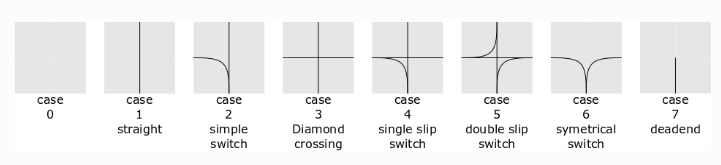
\includegraphics[width=1.0\textwidth]{flatland1}
    \caption{ Tile types in flatland grid \cite{WEBSITE:8} }
    \label{image-myimage2}
\end{figure}

\section {Observations}
In order to solve the flatland environment using RL, we need to decide the observation space and 
action space. Depending on the observation space, we can use different RL algorithms to solve.

\subsection{Global Observation}

Gives a global observation of the entire rail environment.
The observation is composed of the following elements:

\begin{itemize}
    \item Transition map array with dimensions (env.height, env.width, 16), assuming 16 bits encoding of transitions.
    \item Two 2D arrays (env.height, env.width, 2) containing respectively the position of the given agent target and the positions of the other agents targets.
    \item A 3D array (env.height, env.width, 8) with the first 4 channels containing the one hot encoding of the direction of the given agent and the second 4 channels containing the positions of the other agents at their position coordinates.
\end{itemize}

Global observations, specifically on a grid like environment, benefit from the vast research results 
on learning from pixels and the advancements in convolutional neural network algorithms. 
The observation can simply be generated from the environment state and not much additional 
computation is necessary to generate the state.
Also, in this case, when we consider global observation, it is like having a superagent (a 
central controler), which will take action for each of the trains after having the global 
observation.

\subsection{Tree Observations}
Tree observations are local observation that is made for each agent in the environment whenever agent
need to take the action. Also if we consider local observation of each agent then the environment becomes
multiagent, as opposed to the case of global observation.
The tree observation is built by exploiting the \textbf{graph structure of the railway network}. 
The observation is generated by spanning a 4 branched tree from the current position of the agent. 
Each branch follows the allowed transitions until a cell with multiple allowed transitions is reached. 
Here the information gathered along the branch is stored as a node in the tree. This is 
very similar to the observation we made in the previous chapters (in case of scheduling at railway line)
 where the observation is 
the resource information of the resource next to the train and at back to the train.
The figure below illustrates how the tree observation is built:

\begin{figure}[h]
    \centering
    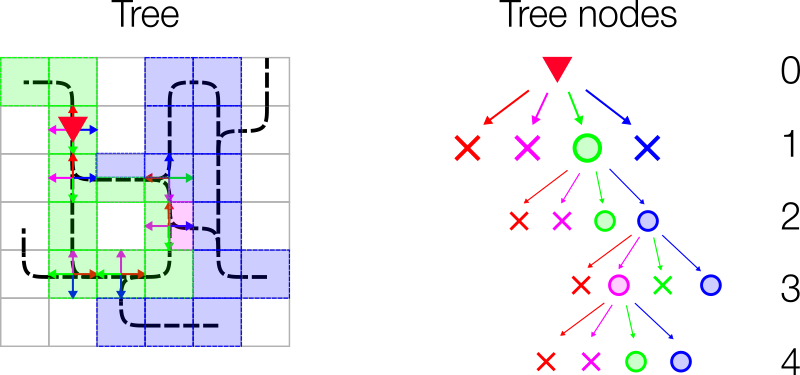
\includegraphics[width=1.0\textwidth]{flatland2}
    \caption{ Tree observation in flatland environment \cite{WEBSITE:8}}
    \label{image-myimage2}
\end{figure}

Each node is filled with information gathered along the path to the node. 
Each node contains 9 features:

\begin {enumerate}
\item If own target lies on the explored branch the current distance from the agent in number of cells is stored.
\item If another agent’s target is detected, the distance in number of cells from the current agent position is stored.
\item If another agent is detected, the distance in number of cells from the current agent position is stored.
\item Possible conflict detected.
\item If an unusable switch (for the agent) is detected we store the distance. An unusable switch is a switch where the agent does not 
have any choice of path, but other agents coming from different directions might.
\item This feature stores the distance (in number of cells) to the next node (e.g. switch or target or dead-end).
\item Minimum remaining travel distance from this node to the agent’s target given the direction of the agent if this path is chosen.
\item Agent in the same direction found on path to node.
\item Agent in the opposite direction on path to node.
\end{enumerate}

\section {Action space}
Thus the actions\cite{WEBSITE:8} of an agent are strongly limited to the railway network. 
This means that in many cases not all actions are valid. The possible actions of an agent are
\begin{enumerate}
    \item 0 \textbf{Do Nothing}: If the agent is moving it continues moving, if it is stopped it stays stopped
    \item 1 \textbf{Deviate Left}: If the agent is at a switch with a transition to its left, 
        the agent will chose th eleft path. Otherwise the action has no effect. 
        If the agent is stopped, this action will start agent movement again if allowed by the 
        transitions.
    \item 2 \textbf{Go Forward}: This action will start the agent when stopped. 
    This will move the agent forward and chose the go strai
    ght direction at switches.
    \item 3 \textbf{Deviate Right}: Exactly the same as deviate left but for right turns.
    \item 4 \textbf{Stop}: This action causes the agent to stop.
\end{enumerate}

\section{Problem Instances}
We can generate different problem instances in the flatland environment, with different railway network 
(sparse as well as dense), different schedules for the agent (trains).
We can also have different speed 
for each agent.
We can also mention the malfunction parameter for each train as this will control the 
rate at which a particular agent malfunctions. Also this will instroduce stochasticity in the environment.
For this work, we will be using three different problem instances as shown in the figure.


\begin{figure}[h]
    \centering
    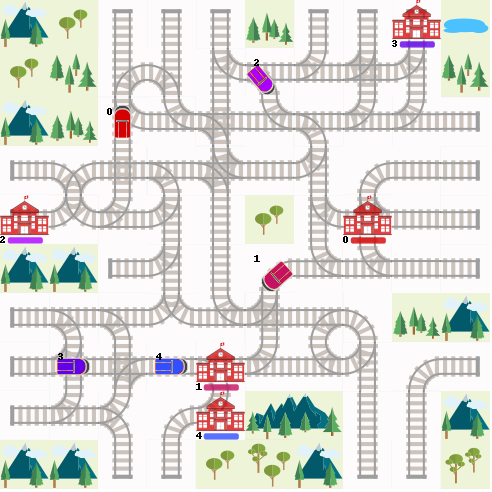
\includegraphics[width=0.5\textwidth]{flatland4}
    \caption{ A random environment. This is a toy example and minimum baseline for the algorithm\cite{WEBSITE:6} }
    \label{image-myimage2}
\end{figure}

\begin{figure}[h]
    \centering
    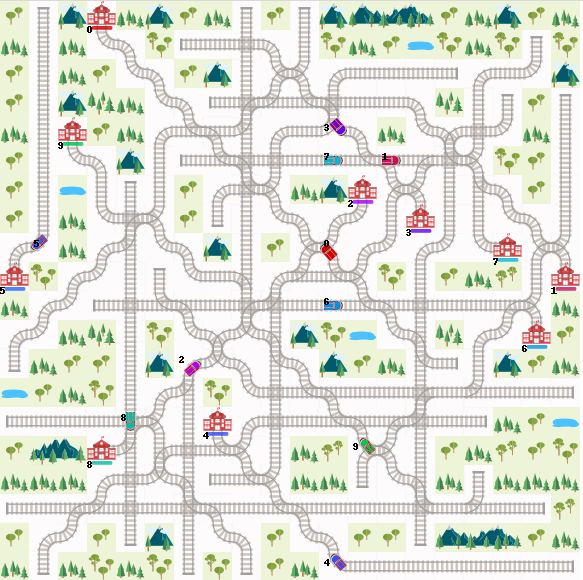
\includegraphics[width=0.5\textwidth]{flatland3}
    \caption{ A complex railway network. Due to the complexity of the network , there are 
    multiple paths from each agent position to their target. Even having multiple paths doen't make 
    this problem instance easy to solve\cite{WEBSITE:6}. }
    \label{image-myimage2}
\end{figure}


\begin{figure}[h]
    \centering
    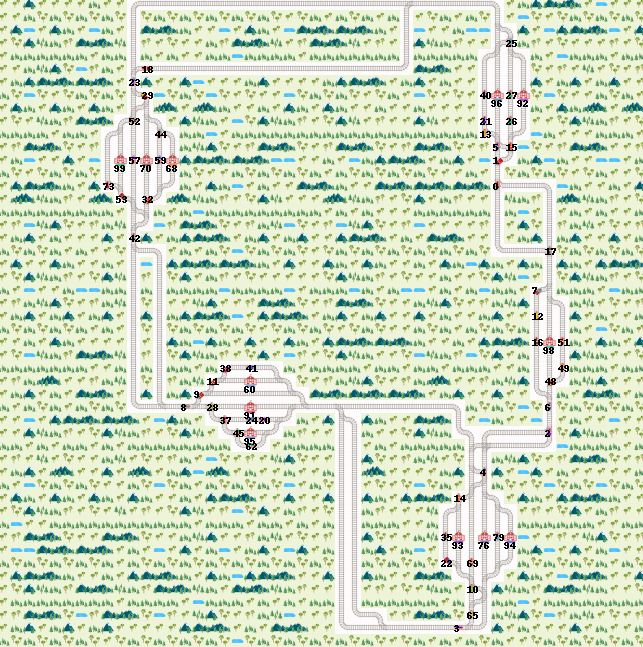
\includegraphics[width=0.8\textwidth]{flatland5}
    \caption{ Real life example.This example have 4 cities (where there are multiple parallel tracks and train targets 
    denoted by red house) each connected by two parallel railway lines. We can add to the complexity by increasing the
    number of cities, decreasing number of parallel track. Also the number of agents in this environment can be large 
    (like 100)\cite{WEBSITE:6} }
    \label{image-myimage2}
\end{figure}

\cleardoublepage
\typeout{}
\chapter{Double deep Q-learning Solution}

We will start this chapter by describing deep Q-learning and then present it's result.

\textbf{Deep reinforcement learning} is the combination of Reinforcement learning and
deep learning. \textbf{Q-learning} is one of the \textbf{off-policy} learning that trains the agent
and tells what is the optimal action to take in each state. This approach can be used
when the number of state-action pairs are limited enough to store there q-value in
the memory. Even if we are able to store q-value of each state-action pair, it is
highly inefficient because the agent need to visit each state-action pair for
reasonable number of times to learn their q-values. Since the total state-action pair
can be very high for real life problems , better approach would be to use the
\textbf{function approximator\cite{BOOK:1}} that approximates the q-value once the state and action are
given as the input. Since neural networks can be used as the function
approximators, so here is the point where deep learning and reinforcement
learning are combined to train the agents to perform in an environment.
In this report, we will be working on DDQN (double deep Q-learning), although there are
whole different class of policy gradient approaches.

\section {Algorithm}

Bellman equation describing the optimal action-value function, $Q^*(s,a)$ is given by,
$$Q^*(s,a) = \mathop{\mathbb{E}}_{s' \sim P}[r(s,a) + \gamma \mathop{\max}_{a'}Q^*(s',a') ]$$

where $s' \sim P$ is shorthand for saying that the next state, s' is sampled by the environment from a 
distribution $P(.|s,a)$

\vspace{\baselineskip}
This Bellman equation is the starting point for learning an approximator to $Q^*(s,a)$. 
Suppose the approximator is a neural network $Q_{\phi}(s,a)$, with parameters $\phi$, 
and that we have collected a set ${\mathcal D}$ of transitions $(s,a,r,s',d)$ (where $d$ 
indicates whether state $s'$ is terminal). We can set up a \textbf{mean-squared Bellman error (MSBE)} function,
 which tells us roughly how closely $Q_{\phi}$ comes to satisfying the Bellman equation:

$$ L (\phi , \mathcal D) = \mathop{\mathbb{E}}_{(s,a,r,s',d) \sim \mathcal D} \left[ \left(Q_{\phi}(s,a) - (r + \gamma(1 - d)\mathop{\max}_{a'} Q_{\phi}(s',a') )\right) ^2 \right] $$ 

When $d==$True , which is to say, when $s'$ is a terminal state—the Q-function should show that the 
agent gets no additional rewards after the current state. 

\vspace{\baselineskip}
Q-learning algorithms for function approximators, such as DQN(and all its variants\cite{ARTICLE:5}, \cite{ARTICLE:6}) are largely based
on minimizing this MSBE loss function. There are two main tricks employed.

\vspace{2.0cm}
\textbf{Trick One : Replay Buffers}
All standard algorithms for training a deep neural network to 
approximate $Q^*(s,a)$ make use of an experience replay buffer. 
This is the set ${\mathcal D}$ of previous experiences. 
In order for the algorithm to have stable behavior, the replay buffer should be large enough to 
contain a wide range of experiences, but it may not always be good to keep everything. 
If you only use the very-most recent data, you will overfit to that and things will break; 
if you use too much experience, you may slow down your learning. We are using a \textbf{buffer replay of size $10^5$}.

\vspace{\baselineskip}
\textbf{Trick Two : Target Networks}. Q-learning algorithms make use of target networks. The term 
$$ r + \gamma(1-d)\mathop{\max}_{a'}Q_{\phi}(s',a')$$

is called the \textbf{target}, because when we minimize the MSBE loss,
 we are trying to make the Q-function be more like this target. 
 Problematically, the target depends on the same parameters we are trying to train: $\phi$. 
 This makes MSBE minimization unstable. The solution is to use a set of parameters which comes close
  to $\phi$, but with a time delay - that is to say, a second network, called the \textbf{target network},
   which lags the first. The parameters of the target network are denoted $\phi_{\text{targ}}$.

\vspace{\baselineskip}
The target network is just copied from the main network every some fixed number of states. In our work,
the target network is updated once per main network update by polyak averaging:
$$ \phi_{\text{targ}} \leftarrow \rho \phi_{\text{targ}} + (1 - \rho)\phi$$
where $\rho$ is a hyperparameter between 0 and 1 (usually close to 1).
\vspace{10cm}
\subsection{Pseudocode}

\begin{algorithm}[h]
    \caption{ Double Deep Q-learning \cite{ARTICLE:5} }
    \begin{algorithmic}
    \State Initialize primary network $Q_{\phi}$ , target network $Q_{\phi_{\text{targ}}}$ , replay buffer  $\mathcal D$,  $\rho \ll 1$
    \State \textbf{for} each Iteration \textbf{do}:
    \State \;\;\;\;\;\;\textbf{for} each environment step \textbf{do}: 
    \State \;\;\;\;\;\;\;\;\;\;\;\;Observe state s and select $a \sim \pi(a,s)$
    \State \;\;\;\;\;\;\;\;\;\;\;\;Execute a in the environment
    \State \;\;\;\;\;\;\;\;\;\;\;\;Observe next state $s'$ , reward r, and done signal d to indicate wether $s'$ is terminal
    \State \;\;\;\;\;\;\;\;\;\;\;\;Store $(s,a,r,s',d)$ in replay buffer $\mathcal D$
    \State \;\;\;\;\;\;\;\;\;\;\;\;If $s'$  is terminal, reset environment state.    
    \State \;\;\;\;\;\;\textbf{for} each update step \textbf{do}
    \State \;\;\;\;\;\;\;\;\;\;\;\;Randomly sample a batch of transitions, $B = {(s,a,r,s',d)}$ from $\mathcal D$
    \State \;\;\;\;\;\;\;\;\;\;\;\;Compute targets
    \State $$Q^*(s,a) \approx r + \gamma (1-d) Q_{\phi}(s' , \mathop{\text{argmax} }_{a'} Q_{\phi_{\text{targ}}}(s',a') )$$
    \State \;\;\;\;\;\;\;\;\;\;\;\; Update Q-function by one step of gradient descent using
    \State $$\nabla_{\phi} \frac {1}{|B|} \sum_{(s,a,r,s',d) \in B} (Q_{\phi}(s,a) - Q^*(s,a)  )^2  $$    
    \State \;\;\;\;\;\;\;\;\;\;\;\; Update target network with
    \State $$ \phi_{\text{targ}} \leftarrow \rho \phi_{\text{targ}} + (1 - \rho)\phi$$
    \end{algorithmic}
    \end{algorithm}
    
\section {Results}
We used DDQN algorithm on flatland environment using tree observation. Although,
it is reasonable to assume that an observation of the full environment is beneficiary for good global solutions. it used to work 
only on small toy examples (even these are hard to train). However, we run into problems when scalability and flexibility
 become an important factor. Already on small toy examples we could show that flexibility quickly becomes an issue
  when the problem instances differ too much. When scaling the problem instances the decision performance of the algorithm 
  diminishes and re-training becomes necessary. On real life instances, we do not believe that a global observation is suited for this 
  problem. So we used DDQN algorithm only on using tree observation.

\vspace{\baselineskip}
In order to use the tree observation, we flat out the tree creating a linear vector whose size depends on tree depth and 
number of features in each node. Since increasing the tree depth increases the size of vector exponentially,
using larger tree depth (of the order of 5,6) can have vector of size of order ($10^4$ to $10^5$).
 In our case we worked on tree depth 2 and 3. Also, we include malfunction (making the problem much harder) in the agents, as this will add 
 stochasticity into the system and helps in better training instance.


 \subsection{Single agent}
 When trained on environment having single agent, the results are very good. This is because, since there is only one 
 agent, the whole environment is stationary with respect to the agent.During the course of training over 2000 episodes on real life example,
 as the training proceeds agent is able to reach the target within time bound ((3*(env.height + env.width)). Moreover, 
 agent is able to find the shortest path as evident from the figure 7.2. Notice that the underlying railway network and
 the schedule of trains (starting position and target) keeps on changing during the course of training. Only certaing specifications
 like number of cities, number of parallel tracks connecting city, number of agents, malfunction rate etc. is fixed.

 \begin{figure}[h]
    \centering
    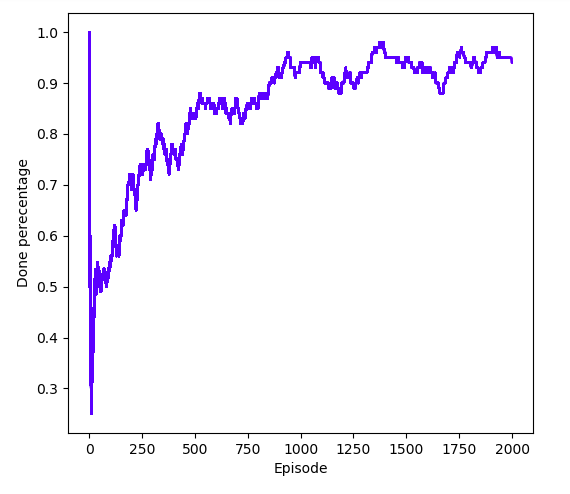
\includegraphics[width=0.5\textwidth]{single_agent_tree_observation_depth2}
    \caption{ Percentage of agents able to complete journey. Single agent, 5 cities, with 2 rails 
    connecting each city with tree depth 2 }
    \label{result10}
\end{figure}

\begin{figure}[h]
    \centering
    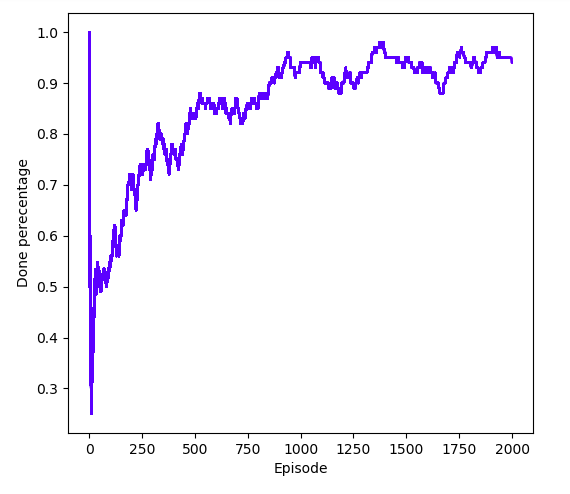
\includegraphics[width=0.5\textwidth]{single_agent_tree_observation_depth2}
    \caption{ Percentage of agents able to complete journey. Single agent, 5 cities, with 2 rails 
    connecting each city with tree depth 2 }
    \label{result10}
\end{figure}

\subsection{Multiple Agent}
The Q-learning algorithm assumes that the environment is stationary for the convergence property. Since in case of multiagent 
environment, environment is non-stationary from the point of view of single agent, so convergence is not guaranteed. 
Although, it is possible that the agent learns what is best possible action for itself given a particular observation but there 
is no way, agent can cooperate perfectly. 

\begin{figure}[H]
    \centering
    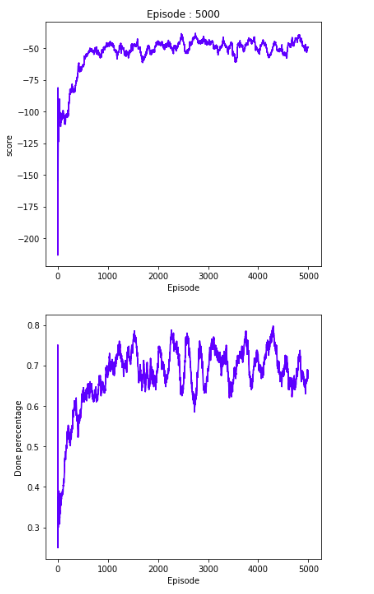
\includegraphics[width=0.5\textwidth]{agent4_city_3_multi}
    \caption{Result of training over real life railway network with 4 agents, 3 cities and tree depth 2 for 5000 episodes. 
        (A) Score of agent, this shows the average reward of agents as the training progresses. 
        (B) Percentage of agents able to complete journey as the training progresses. }
    \label{result10}
\end{figure}

The result shows that, 80\% of the agents are able to complete there journey using short paths when railway network have 4 agents, 3 cities. 
So the results are good when the number of agents is small (in this case 4).

\begin{figure}[H]
    \centering
    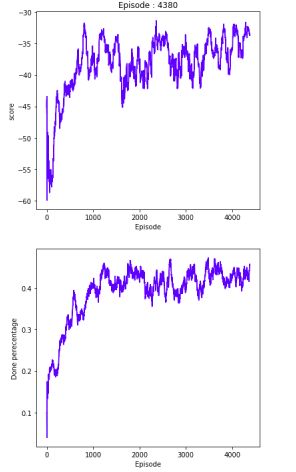
\includegraphics[width=0.5\textwidth]{agent10_city3_multi}
    \caption{Result of training over real life railway network with 10 agents, 3 cities and tree depth 2. 
        (A) Score of agent, this shows the average reward of agents as the training progresses. 
        (B) Percentage of agents able to complete journey as the training progresses. }
    \label{result10}
\end{figure}

So as the number of agents increases to 10, with everything else same, only 40\% of the agents are able to complete there
journey. The results are even worse, when the number of agents increases more.

\section{Alternate RL algorithms}
Q-learning algorithm is designed having the assumption that the environment is stationary with respect to the 
agent. But in case of multiagent environment, environmnent is non stationary with respect to the agent, violating Markov assumptions required for 
convergence of Q-learning. There are RL algorithms for multiagent environment. One of the most effective is 
\textbf{Multi-Agent Actor-Critic for Mixed
Cooperative-Competitive Environments (MADDPG)\cite{ARTICLE:7}} based on actor critic based approach for single agent. 
In the next chapter, we will solve the same problem using cooperative path finding. 
\cleardoublepage
\typeout{}
\chapter{Cooperative Pathfinding}

In this chapter, we will try to solve the problem using \textbf{Cooperative pathfinding}\cite{ARTICLE:8}.
There are some drawbacks related to this approach that we will see at the end of chapter and 
ways to resolve it.
When a single unit pathfinds through a map, basic A* search is perfectly adequate. But
when multiple units are moving at the same time, this approach can break down, often
with frustrating consequences for the player.

\section{The problem with A*}
A* search is used to find
the shortest path to the destination for each unit (agent in case of flatland environment). This search ignores the
presence of other units, or perhaps treats them as stationary obstacles. If a collision is
imminent, the units involved will re-search and select a new path.

\vspace {\baselineskip}
In case of \textbf{cooperative pathfinding}, A* search is still used, but in a way that takes account of other
agents’ movements. The only requirement is that agents can communicate their planned paths which is always
possible in case of flatland environment. This is generally
most appropriate for agents on the same side; agents 
units will not usually be so cooperative. 
Non-cooperative pathfinding raises the tricky issue of path prediction, and
isn’t discussed here as it is not applicable to our flatland problem.

\section{The Fourth Dimension}
To tackle the cooperative pathfinding problem, the search algorithm needs to have full
knowledge of both obstacles and agents. However, when agents move around there is no
satisfactory way to represent their routes on a stationary map. To overcome this problem,
we extend the map to include a fourth dimension: time. We will call the original map the
space map and the new, extended map the space-time map.
The \textbf{space map} consists of a three-dimensional grid of
locations and orientation (x, y,orientation). The \textbf{space-time} map consists of a four-dimensional grid
of cells: Cell(x, y, orientation, t).

\vspace{\baselineskip}

In flatland environment, agent have 5 actions: do nothing, deviate left (if possible), go forward, deviate right (if possible), stop.
Executing forward (when the agent is facing North) corresponds to moving a agent through the space-time map from
Cell(x, y, North , t) to Cell(x, y + 1, North , t + 1).All five actions have a cost
of one, corresponding to their duration. Once the agent reaches the target, agent will 
disappear. A* search can now be used on the space-time map. The goal of the agent is to reach the
destination at any time. A* will find the route that achieves this goal with the lowest cost.

\section{Reservation Table}
Once a agent has chosen a path, it needs to make sure that other agents know to avoid the
cells along its path. This is achieved by marking each agent into a \textbf{reservation table}. This is
a straightforward data structure containing an entry for every cell of the space-time map \textbf{excluding the orientation}.
Each entry specifies whether the corresponding cell is available or reserved. Once an
entry is reserved, it is illegal for any other agent to move into that cell. The reservation acts
like a transient obstacle, blocking off a location for a single time-step in the future.

\vspace{\baselineskip}
Using a reservation table and a space-time map, we are able to solve the cooperative
pathfinding problem. Each agent pathfinds to its destination using space-time A*, and then
marks the path into the reservation table. Subsequent agents will avoid any
reserved cells, giving exactly the coordinated behavior that we desire.
Note, a cell is reserved when some location is occupied at some time. Orientation does not have 
any role here.

\begin{figure}[h]
    \centering
    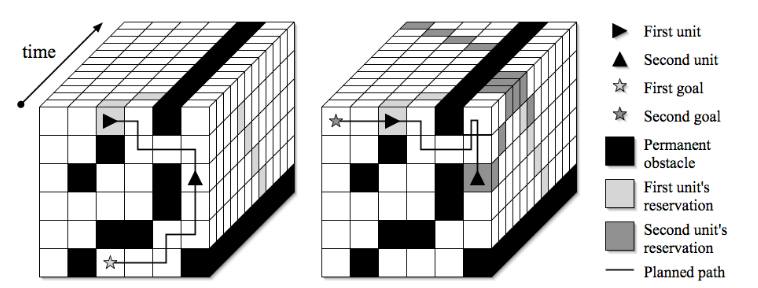
\includegraphics[width=1.0\textwidth]{Cooperative1}
    \caption{ Two agents pathfinding cooperatively. (A) The first agent searches for a path and
    marks it into the reservation table. (B) The second agent searches for a path, taking account
    of existing reservations, and also marks it into the reservation table. Orientation is not shown in 
    this example.\cite{ARTICLE:8}}
    \label{image-myimage2}
\end{figure}

We are reserving one cell in the reservation table for the agent. But it can lead to deadlock when executing.
Unfortunately, this way of using the reservation table doesn’t prevent two agents crossing
through each other, head to head. If one agent has reserved (x, y, t) and (x + 1, y, t + 1),
there is nothing to stop a second agent from reserving (x + 1, y, t) and (x, y, t + 1). Note orientation 
is not used in case of reservation table. This
problem can be avoided by making \textbf{two reservations} for each location involved in the
action, one at time t and one at time t + 1. Alternatively, head to head collisions can be
explicitly identified and marked as illegal actions. We will be making two reservations for each location 
in our work as it is able to avoid the deadlock completely. We now have a complete algorithm for cooperative pathfinding.

\section{Choosing heuristic}
The performance of A* depends upon the choice of heuristic. With the search space
extended by an extra dimension, the choice of heuristic becomes even more important.

\subsection{Manhattan distance heuristic}
For grid-based maps, the Manhattan distance is often used as a heuristic. It is simply the
sum of the x and y distances to the destination. It provides a good estimate of the time to
reach the destination on an open map. However, if the shortest path to the destination is
circuitous, then the Manhattan distance becomes a poor estimate.

\vspace{\baselineskip}
During A* search, new locations are kept on the open list and explored locations are kept
on the closed list. At each step, the most promising location is selected from the open list
according to its f value. The f value estimates the total distance to the destination, passing
through that location. It is the sum of g, the distance traveled by A* to reach the location,
and h, the heuristic distance from the location to the destination.

Using the Manhattan distance heuristic, many locations on the map can have an f value
that is less than the true distance to the destination. For example, the map in given figure (not showing orientation dimension 
to make things simple)
shows the f values for all locations visited by spatial A*. Almost the entire map has been
explored before the destination is found, a phenomenon known as \textbf{flooding}.

\begin{figure}[h]
    \centering
    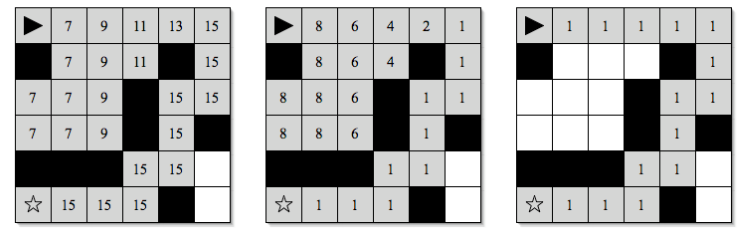
\includegraphics[width=1.0\textwidth]{cooperative2}
    \caption{The Manhattan distance heuristic can be inefficient. (A) Flooding occurs in
    spatial A* when the f values (shown) at many locations are lower than at the destination.
    (B) The number of visits to each location (shown) can be high during space-time A*. (C)
    Using the true distance heuristic, the number of visits to each location (shown) is optimal.\cite{ARTICLE:8}}
    \label{image-myimage2}
\end{figure}

Now consider what happens if we use the Manhattan distance in a space-time map.
Again, it will work well on an open map. But take a look at the equivalent map in Figure, which shows
 the number of times each location is explored by space-time A*. Not
only will space-time A* explore many more locations at the time of each deviation, it will
explore those locations at later times too. This is because pausing, or returning to a
previous location, appears more promising than moving away from the destination. In
other words, \textbf{the problem has been magnified many times}.

\subsection{True distance heuristic}
We will use true distance heuristic as our heuristic for space-time search. True distance heusristic is 
the shortest distance to the destination, taking account of obstacles, but ignoring agents.
True distance from each location and orientation to each target is pre calculated and stored to make the 
algorithm faster. When using true distance heuristic in case of cooperative pathfinding, the algorithm is 
known as \textbf{Hierarchical Cooperative A*}

\subsubsection{Consistency}
An admissible heuristic never overestimates the distance to the goal. A* search with an
admissible heuristic is guaranteed to find the shortest path. However, there is a stronger
property, known as consistency. A \textbf{consistent heuristic maintains the property
h(A) $\leq$ cost(A, B) + h(B) between all locations A and B}. In other words, the estimated
distance doesn’t jump around between the locations along a path. Both manhattan and true distance heuristic
are consistent.


\section{Results}
We implemented the cooperative A* (both manhattan and true distance heuristic) on flatland environment 
having both only one cell reserved (at time t) and two cell reserved (at time t and t+1).

\subsection{Cooperative A* with only cell reserved at t}
When only one cell is reserved at time t, the results are very bad as \textbf{most of the agents ended in 
deadlock}. In case of problem instance 1, only 2 out of 10 agents completed their journey. Rest ended in deadlock.
In case of problem instance 2, 13 out of 20 agents completed their journey. This is still high because problem 
instance 2, have multiple paths from each location and orientation to there target.
In case of problem instance 3 (real life example), only 6 out of 100 agents are able to complete journey.
Clearly, this algorithm is not good. 

\subsection{Cooperative A* with cell reserved at t and t+1}
The results in this case are very good, as all the agents are able to complete their journey with great cooperation.
I am attaching a video showing the great cooperation between agents. One thing to notice is \textbf{path length}
for each agent after they complete their journey. In case of problem instance 1, agents 6 and 8 take much larger path
compared to shortest path. In case of problem instance 2, since there are so many paths from given location 
and orientation to the target, actual path taken by the agent and shortest path are almost of same length.
In case of problem instance 3 (real life example), as the agent number increases they take longer and longer routes.
This is because the agent with less order number have already made reservations and agent with higher order number 
have to take alternate path other than the best path. In fact the extent of deviation from the 
shortest path shows the cooperation between the agents. So, with agent with less order number have 
\textbf{higher priority}. So we can assign priority to the trains based on there order number.
Although this is not very good.
\begin{figure}[h]
    \centering
    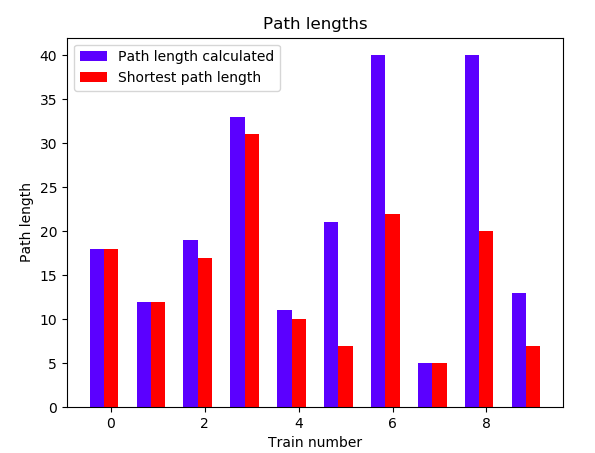
\includegraphics[width=0.5\textwidth]{cooperative3}
    \caption{Pathlength (problem instance 1)}
    \label{image-myimage2}
\end{figure}

\begin{figure}[h]
    \centering
    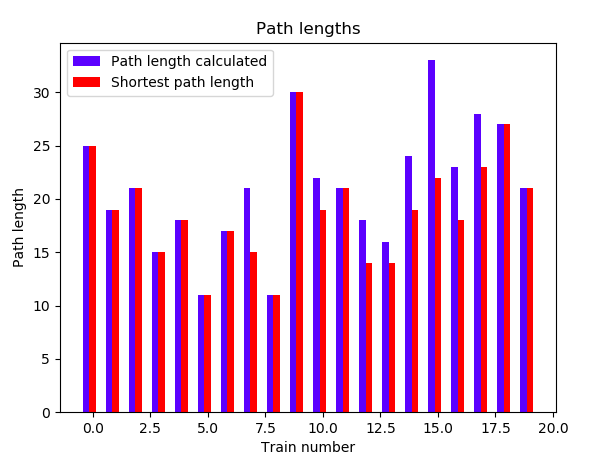
\includegraphics[width=0.5\textwidth]{cooperative4}
    \caption{Pathlength (problem instance 2)}
    \label{image-myimage2}
\end{figure}

\begin{figure}[H]
    \centering
    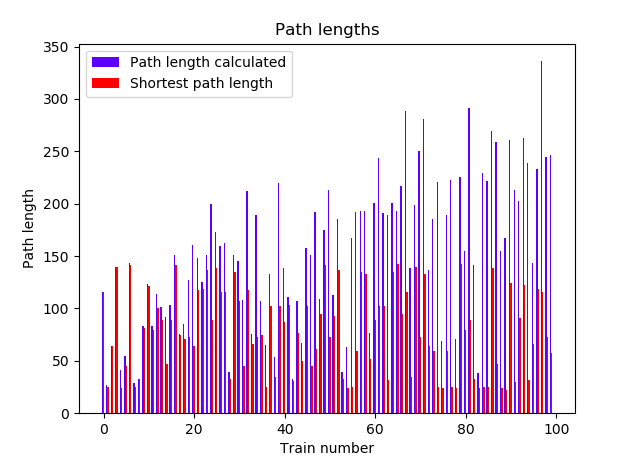
\includegraphics[width=0.8\textwidth]{cooperative5}
    \caption{Pathlength (problem instance 1)}
    \label{image-myimage2}
\end{figure}

\section{Drawbacks}
Hierarchical cooperative A* works really good on flatland environment, but this algorithm is deterministic.
This mean, if we include stochasticity into the system, by making agent malfunction, this algorithm is likely 
to break. To solve this issue, instead of finding the path upto the target, agent can find path upto certain 
depth and then once completed that depth, can resume search. This will be more robust to stochasticity in 
environment. This algorithm is called \textbf{Windowed Hierarchical cooperative A* (WHCA)}.
Also, in Hierarchical cooperative A*, priority is already introduced depending on the agent order. This can be resolved searching 
the path upto fixed depth, follow the path and then change order. This way each agent will have higher priority at some point 
of time and hence resolving the issue. We can also try to combine this algorithm with some RL algorithm to make it 
more robust to the environment with high stochasticity.
\cleardoublepage
\typeout{}
\chapter{Conclusion and Future Work}

So far, focus is to fully understand the problem statement, what are the variations of the 
problem and then how RL algorithms can be used to solve this problem. The report discusses
two approach, to solve the problem. Currently the focus is to implement the prior approach and
see how good it is working, how good it is scaling to real life problem instances, how good it is 
performing compared to the present approaches and how to improve upon it. For the implementation of the 
algorithm, we need to implement the discrete railway simulator. For that, I have gone through the NetworkX and SimPy 
packages of standard python. The future plan is to complete the implementation of the simulator and then test 
our proposed method on the simulator.

Since we are tackling blocking version of the JSSP problem, so the approach that we will 
develop can be used to solve the JSSP problem with reasonable approximation. So the future plan is also 
to use the developed approaches on other similar problems as well.

\cleardoublepage
\bibliography{btp}
\bibliographystyle{IEEEtran}

\end{document}

